\documentclass[a4paper,10pt]{article}

\usepackage[a4paper,margin=1in]{geometry}
\usepackage{multicol}      
\usepackage{graphicx}      
\usepackage{parskip}       
\usepackage{titlesec}       
\usepackage{mathptmx}
\usepackage{amsmath}
\usepackage{subcaption}
\usepackage{float} 
\usepackage{amsmath,amssymb}
\usepackage[authoryear]{natbib}
\usepackage[colorlinks=true, citecolor=blue, linkcolor=black, urlcolor=blue]{hyperref}


\titleformat{\section}{\large\bfseries}{\thesection}{1em}{}
\titleformat{\subsection}{\normalsize\bfseries}{\thesubsection}{1em}{}

\begin{document}

\begin{center}
    {\Large \textsc{Disentangling the Components of the Milky Way}}\\[0.2cm]
    {\textsc{Inferring the Structure of the Milky Way in Phase-Space Using Gaussian Mixture Modelling with Extreme Deconvolution}}\\[0.2cm]
    Raunaq Singh Rai \quad | \quad MPhil Data Intensive Science \quad | \quad University of Cambridge
\end{center}

\begin{multicols}{2}
% Start of two-column content

\section*{Motivation and Scientific Justification}

An important question in Galactic Archaeology is \emph{when} the Milky Way’s disc first settled.  
Standard models suggest that the disc formed relatively late, after the interstellar medium had been enriched by multiple generations of stars \cite{Sestito2020} \cite{Gurvich2023}. 
This implies a lack of stars with disc-like kinematics at very low metallicities. 
Since metallicity generally increases over cosmic time, it can be used as a rough proxy for stellar age: lower metallicity stars are typically older, having formed when the Galaxy was less chemically evolved. 
Thus, identifying a coherent, metal-poor disc population would challenge the \emph{late-disc} paradigm and force a reassessment of the balance between in-situ star formation and accreted growth.

Zhang et al.\ (2024)~\cite{zhang2024existencemetalpoordiscmilky} addressed this question by applying Extreme-Deconvolution Gaussian Mixture Modelling (XD-GMM) to the full $(v_{\phi},v_{R},v_{Z})$ phase-space of 
Gaia DR3 bright red giant stars, and found no evidence for a cold, rotation-supported disc at very low metallicity. However, their analysis did not account for $\alpha$ abundance, which can serve as a tracer of star-formation timescales.

We reproduce their metallicity-binned XD-GMM using the same bright RGB catalogue, and extend the work by dividing stars into high and low $\alpha$ sequences following Viswanathan et al.\ (2024)~\cite{Vis2024}.  
Within each $\alpha$ branch, we perform XD-GMM fits in successive metallicity bins, selecting the optimal number of components via the Bayesian Information Criterion.  
By inspecting the weights and kinematic properties of these components, we assess whether the disc-like signatures for the high and low $\alpha$ sequences emerge at different metallicities in line with current understanding.


\section*{Methodology}

After data cleaning and processing, the velocity distribution $(v_R, v_\phi, v_z)$ is modelled using Extreme-Deconvolution Gaussian Mixture Modelling (XD-GMM) \cite{Bovy2011}\cite{pygmmis}, 
which accounts for observational uncertainties. We bin stars by metallicity and use the Bayesian Information Criterion (BIC) to determine the 
number of Gaussian components per bin. This allows us to identify structure without over fitting and introducing too many gaussians.


We extend the original method by splitting the sample into high and low $\alpha$ sequences \citep{Vis2024}, fitting separate 
XD-GMMs to each. By inspecting the component weights and kinematic properties, we quantify the emergence of rotational support 
and assess the presence of disc-like populations across both chemical tracks.

Following this, to determine the presence of disc-like kinematics, we compute the ratio of azimuthal velocity $v_\phi$ and its 
dispersion $\sigma_\phi$ for each component: a ratio approximately above 3 is considered to be disk-like. 
We then move to perform residual analysis to test whether disc-like kinematics are present
but are too weak to be detected by XD-GMM.

\section*{Key Findings}

\begin{figure}[H]
  \centering
  \begin{subfigure}[t]{0.24\linewidth}
    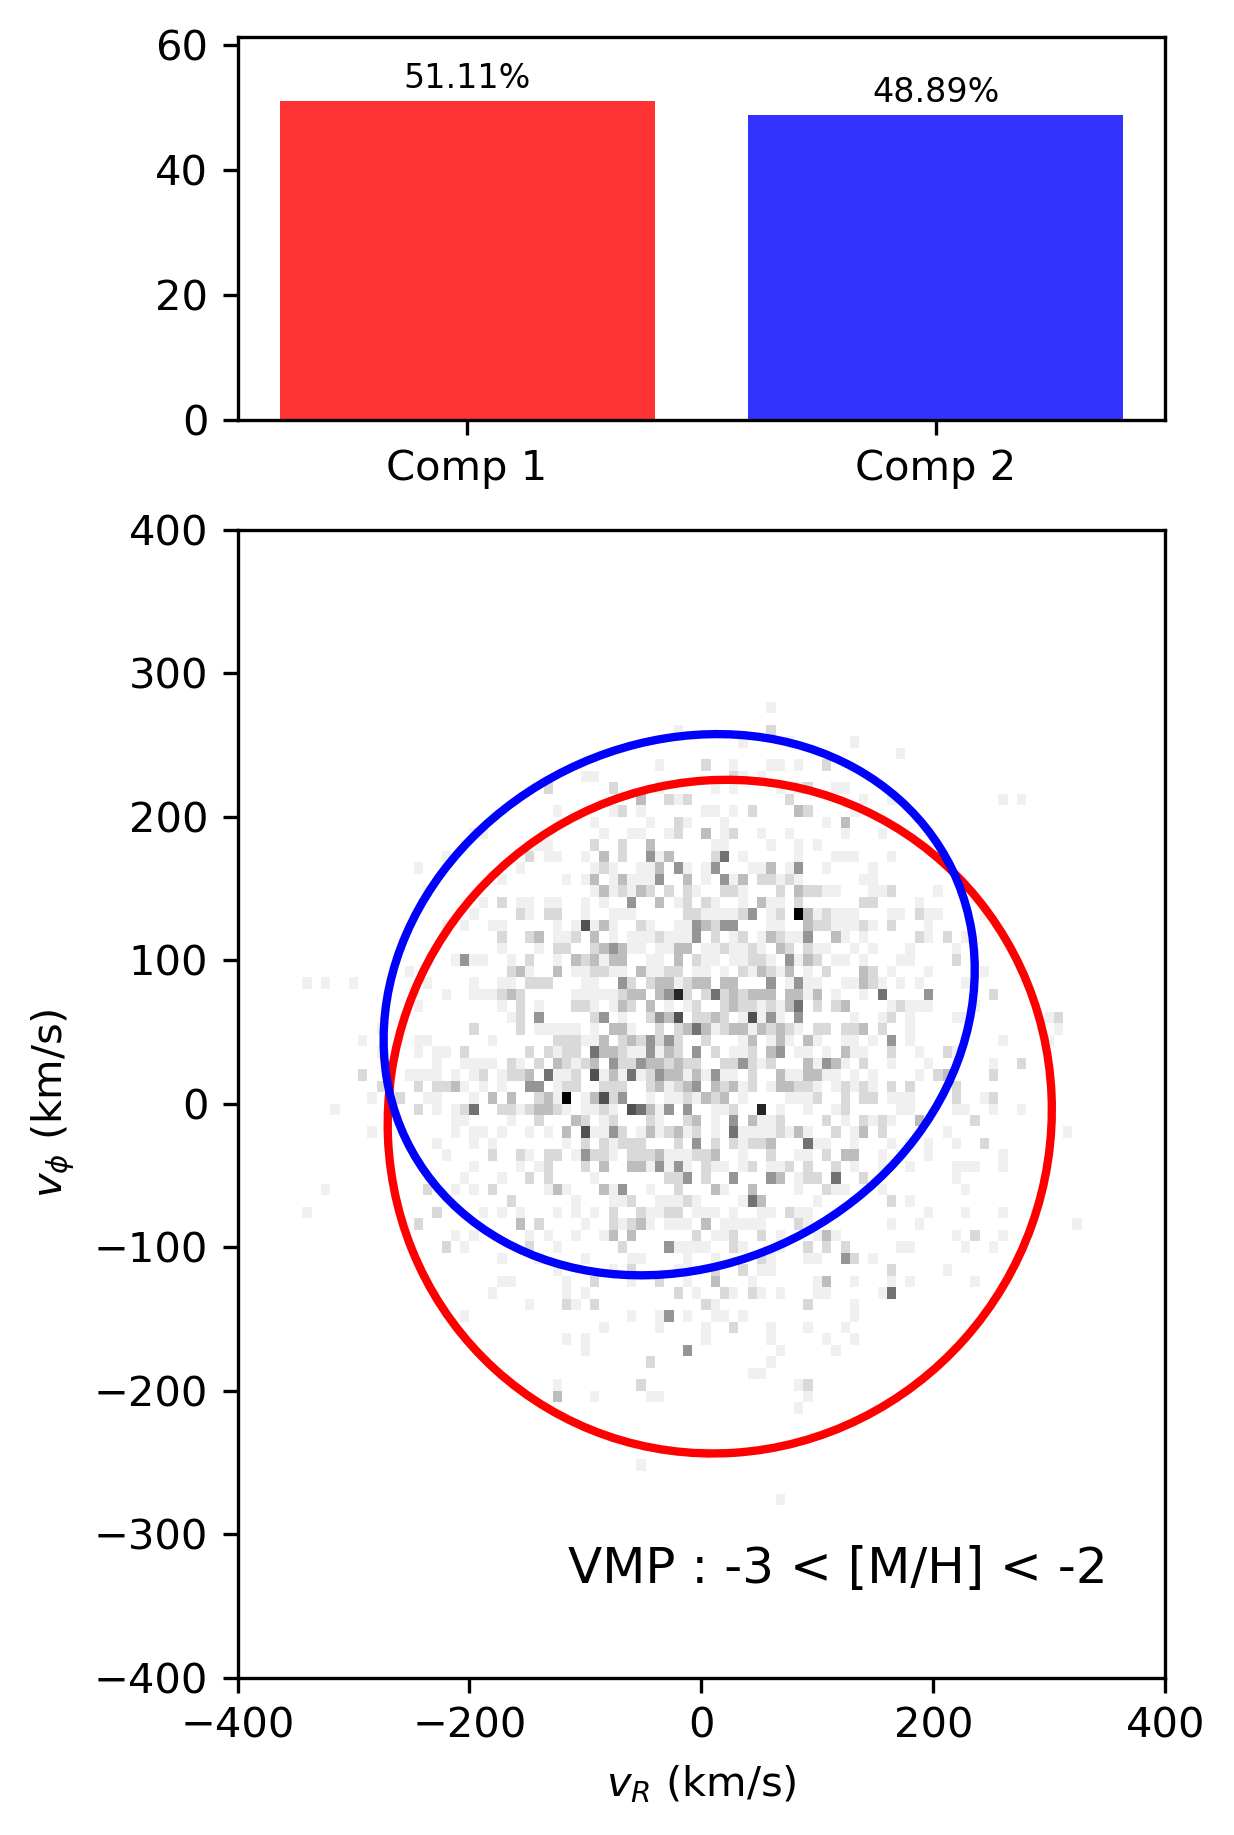
\includegraphics[width=\linewidth]{../figures/gmm_VMP.png}
    \caption{\href{https://raw.githack.com/raunaq-rai/Disentangling-the-Milky-Way-using-GMM/main/figures/VMP\_\_-3\%5BM\_H\%5D-2.html}{VMP}}
    \label{fig:gmm_vmp}
  \end{subfigure}\hfill
  \begin{subfigure}[t]{0.24\linewidth}
    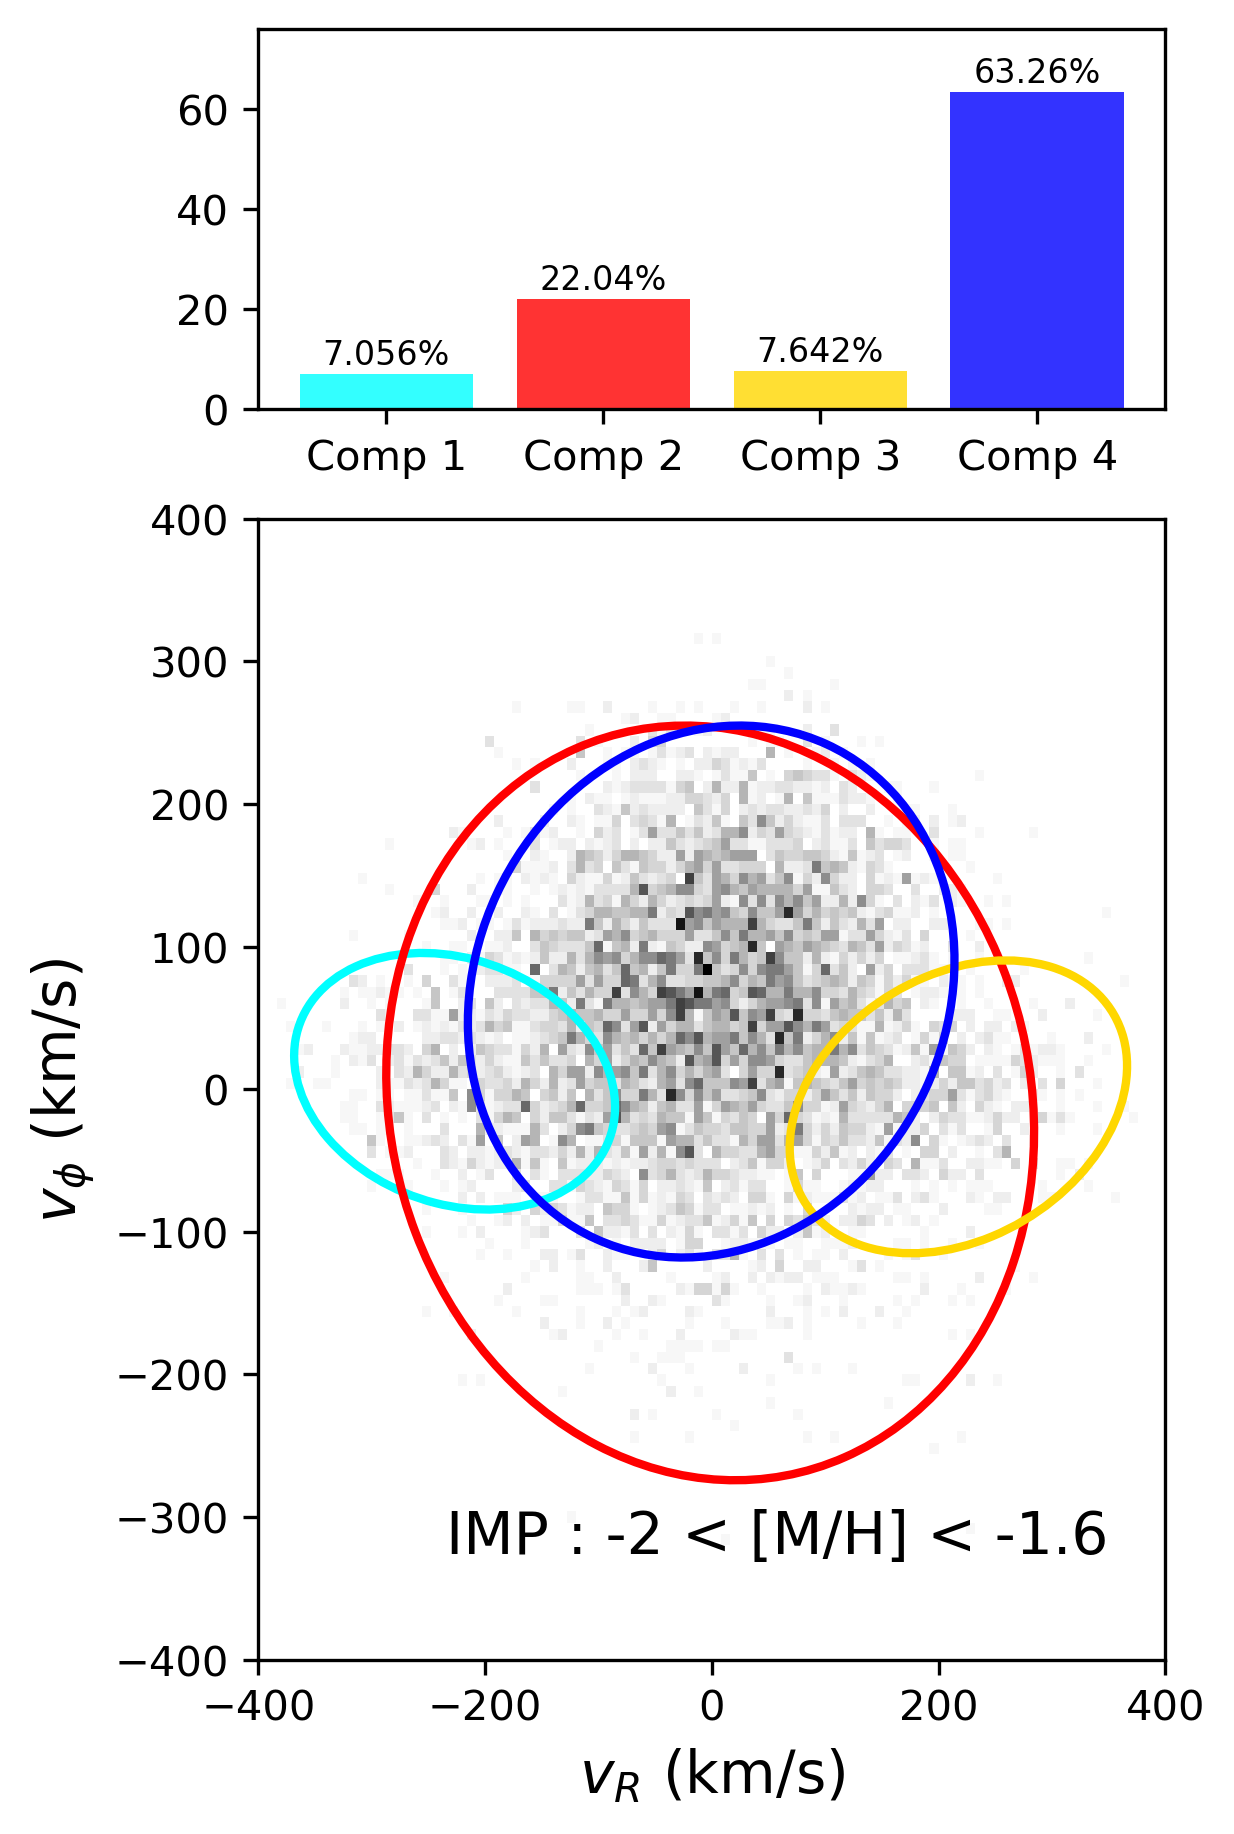
\includegraphics[width=\linewidth]{../figures/gmm_IMP.png}
    \caption{\href{https://raw.githack.com/raunaq-rai/Disentangling-the-Milky-Way-using-GMM/main/figures/IMP\_\_-2\%5BM\_H\%5D-1.6.html}{IMP}}
    \label{fig:gmm_imp}
  \end{subfigure}\hfill
  \begin{subfigure}[t]{0.24\linewidth}
    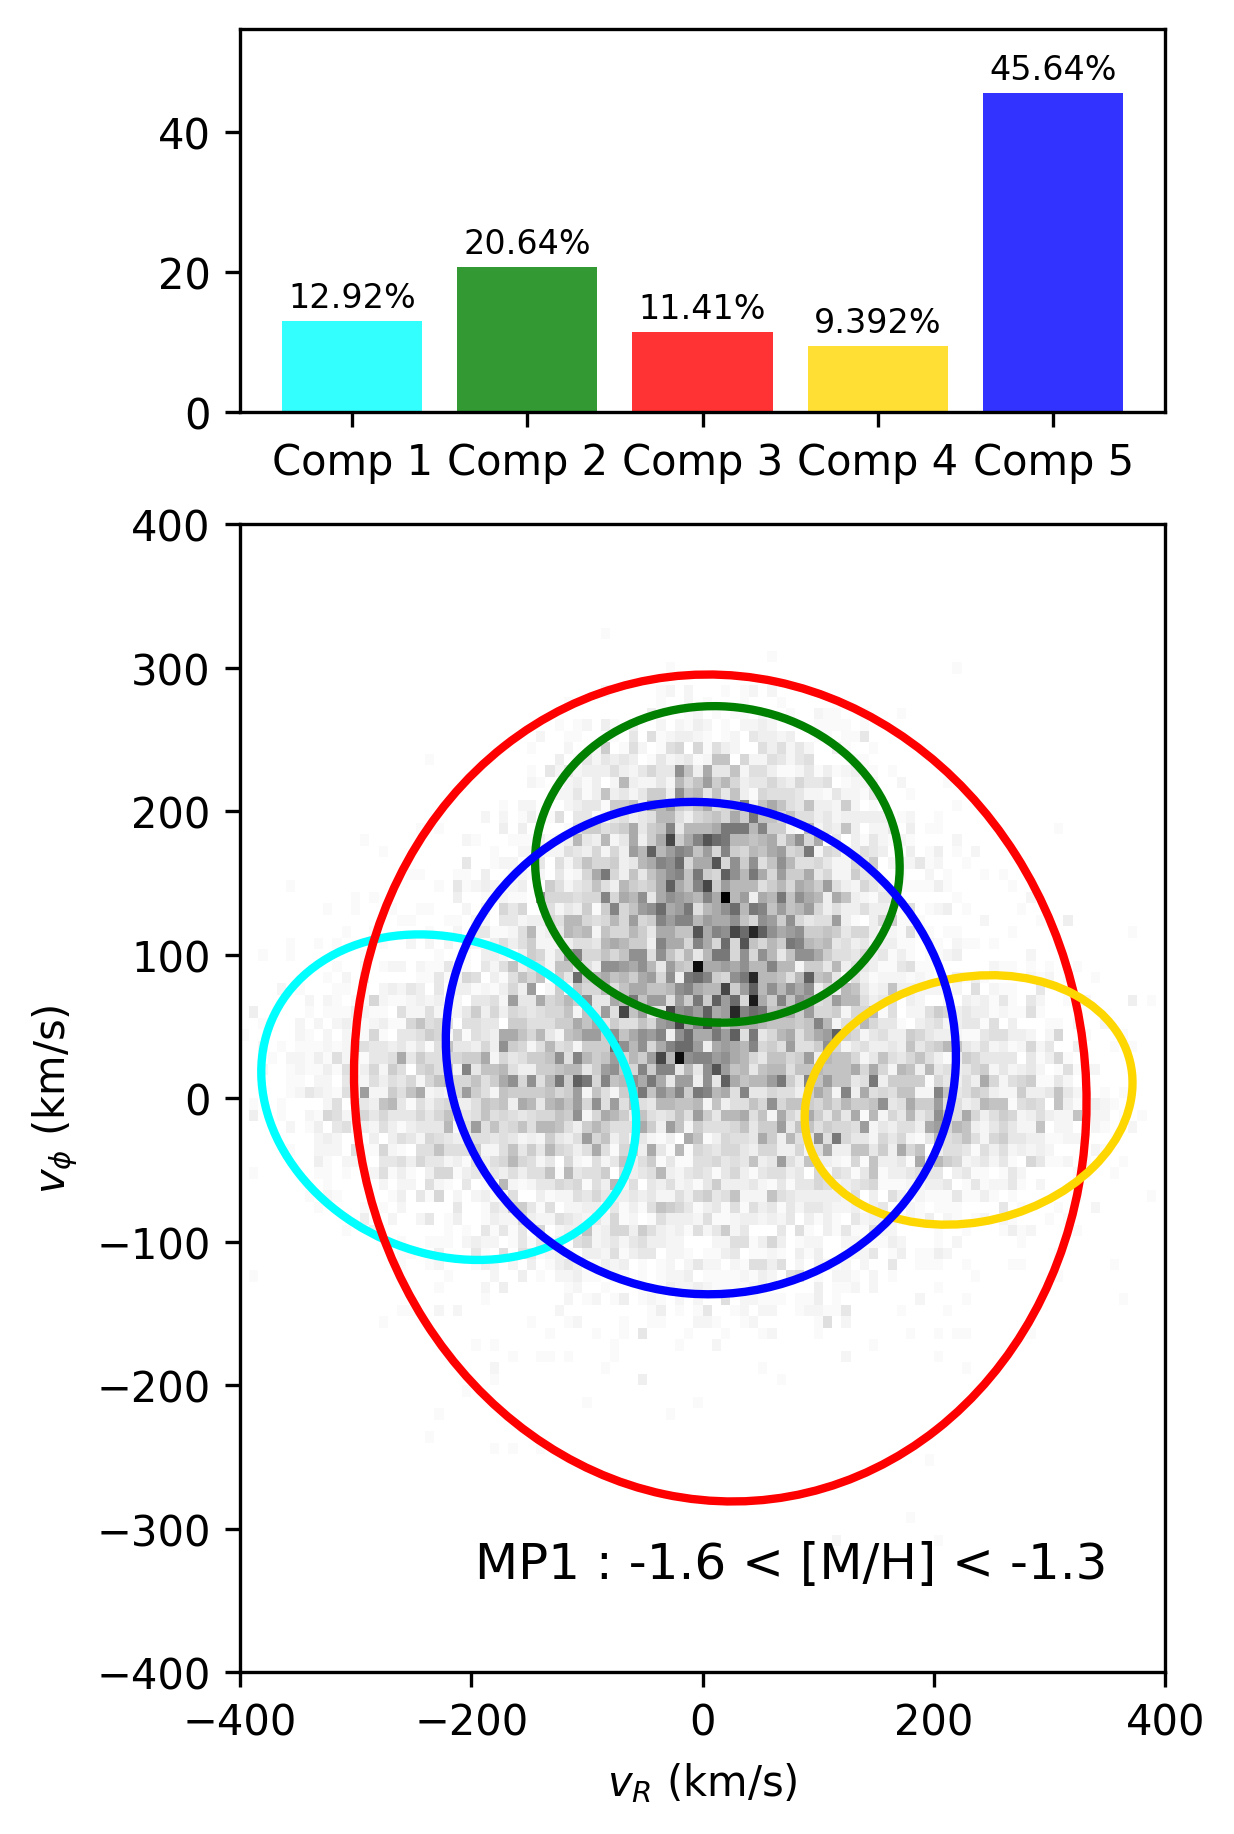
\includegraphics[width=\linewidth]{../figures/gmm_MP1.png}
    \caption{\href{https://raw.githack.com/raunaq-rai/Disentangling-the-Milky-Way-using-GMM/main/figures/MP1\_\_-1.6\%5BM\_H\%5D-1.3.html}{MP1}}
    \label{fig:gmm_mp1}
  \end{subfigure}\hfill
  \begin{subfigure}[t]{0.24\linewidth}
    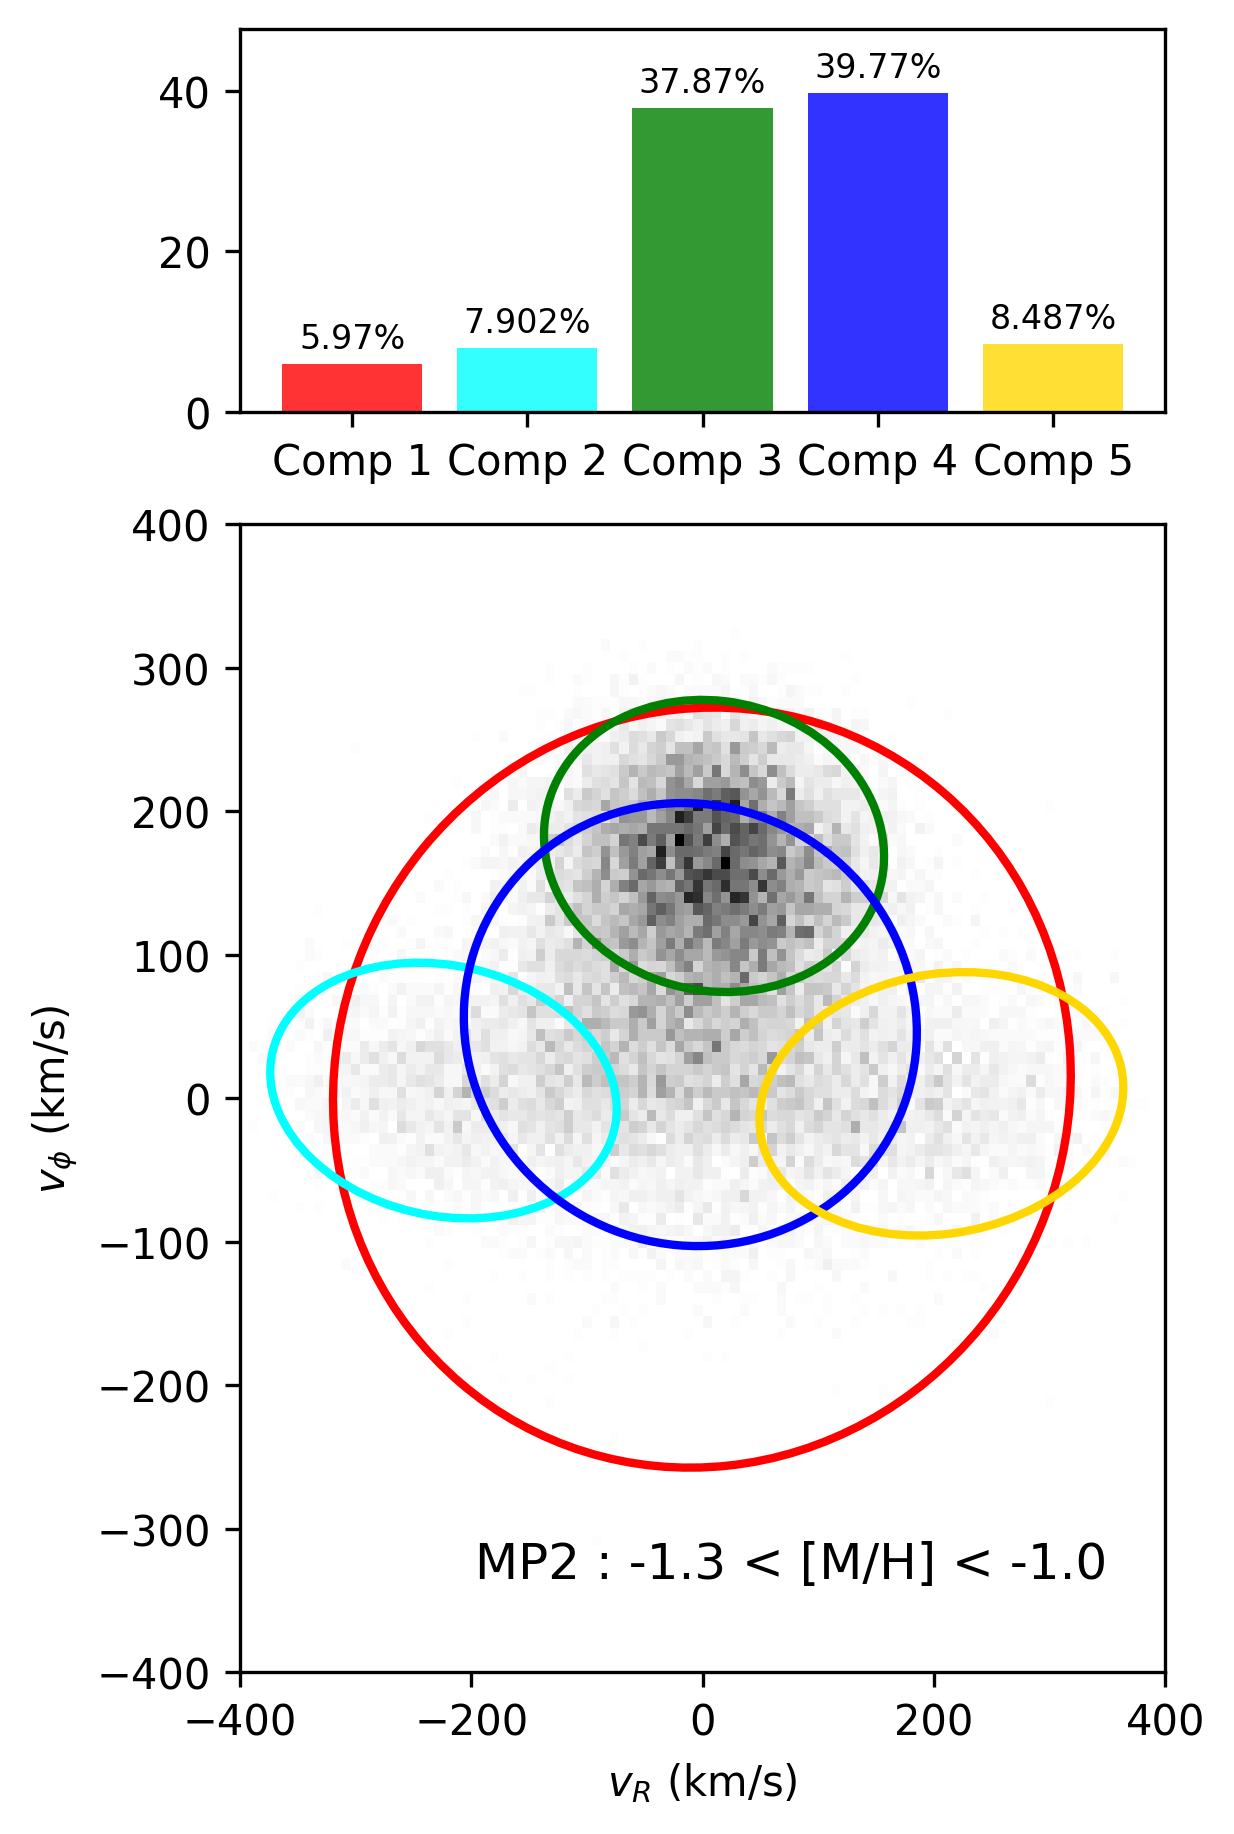
\includegraphics[width=\linewidth]{../figures/gmm_MP2.png}
    \caption{\href{https://raw.githack.com/raunaq-rai/Disentangling-the-Milky-Way-using-GMM/main/figures/MP2\_\_-1.3\%5BM\_H\%5D-1.0.html}{MP2}}
    \label{fig:gmm_mp2}
  \end{subfigure}

  \caption{XD-GMM decomposition of red giant kinematics across metallicity bins. Links to the fully interactive 3-D plots for each bin are provided in the subcaptions.}
  \label{fig:gmm_zhang}
\end{figure}


Below $\mathrm{[M/H]} \sim -2$, no disc-like component is detected. The kinematics are fully 
explained by two broad halo Gaussians: one stationary and one mildly prograde likely associated 
with the Aurora population~\cite{Belokurov2022}. In the intermediate metallicity bin, two 
additional highly radial, non-rotating components emerge, linked to the 
Gaia-Sausage/Enceladus (GS/E) merger~\cite{Belokurov2018}. These represent remnants of a 
major head-on collision between the Milky Way and a massive dwarf galaxy, which deposited stars 
on radial orbits and contributed significantly to the inner halo's anisotropic structure.

Disc-like rotation first appears at $\mathrm{[M/H]}\gtrsim-1.6$, where a thick-disc 
component (approximately $22\%$ of stars) rotates at $\langle v_\phi\rangle\approx160\ \mathrm{km\,s^{-1}}$ 
with $\sigma_\phi\approx57\ \mathrm{km\,s^{-1}}$ ($V_{\rm rot}/\sigma_\phi\approx2.8$, just 
below the “discy” threshold of $\sim3$). As metallicity increases to the MP2 bin, this component 
grows to $37.4\%$ of the sample and surpasses the discy criterion with 
$V_{\rm rot}/\sigma_\phi\approx3.5$, indicating a well-established, rotation-supported thick disc.  



Monte Carlo residual analysis in the VMP and IMP bins detects only minor excesses, 
constraining any hidden low-metallicity disc to at most $\sim1\%$ of the sample. Together, these diagnostics suggest the 
absence of a disc below $\mathrm{[M/H]}\sim-1.6$).  


Following Viswanathan et al.~\cite{Vis2024}, we split the sample into high- and low-$\alpha$ sequences—proxies for 
rapid versus extended star-formation timescales. Figure~\ref{fig:mh_vphi_alpha} shows that high-$\alpha$ stars 
spin up gradually, with $\langle v_\phi\rangle$ rising and $\sigma_\phi$ falling steadily from 
$\mathrm{[M/H]}\!\sim\!-2$ to $-1$, whereas the low-$\alpha$ branch remains dispersion-dominated until a 
sharp transition at $\mathrm{[M/H]}\sim-1.3$, when disc kinematics abruptly appear.  

\begin{figure}[H]
  \centering
  \begin{subfigure}[t]{0.48\linewidth}
    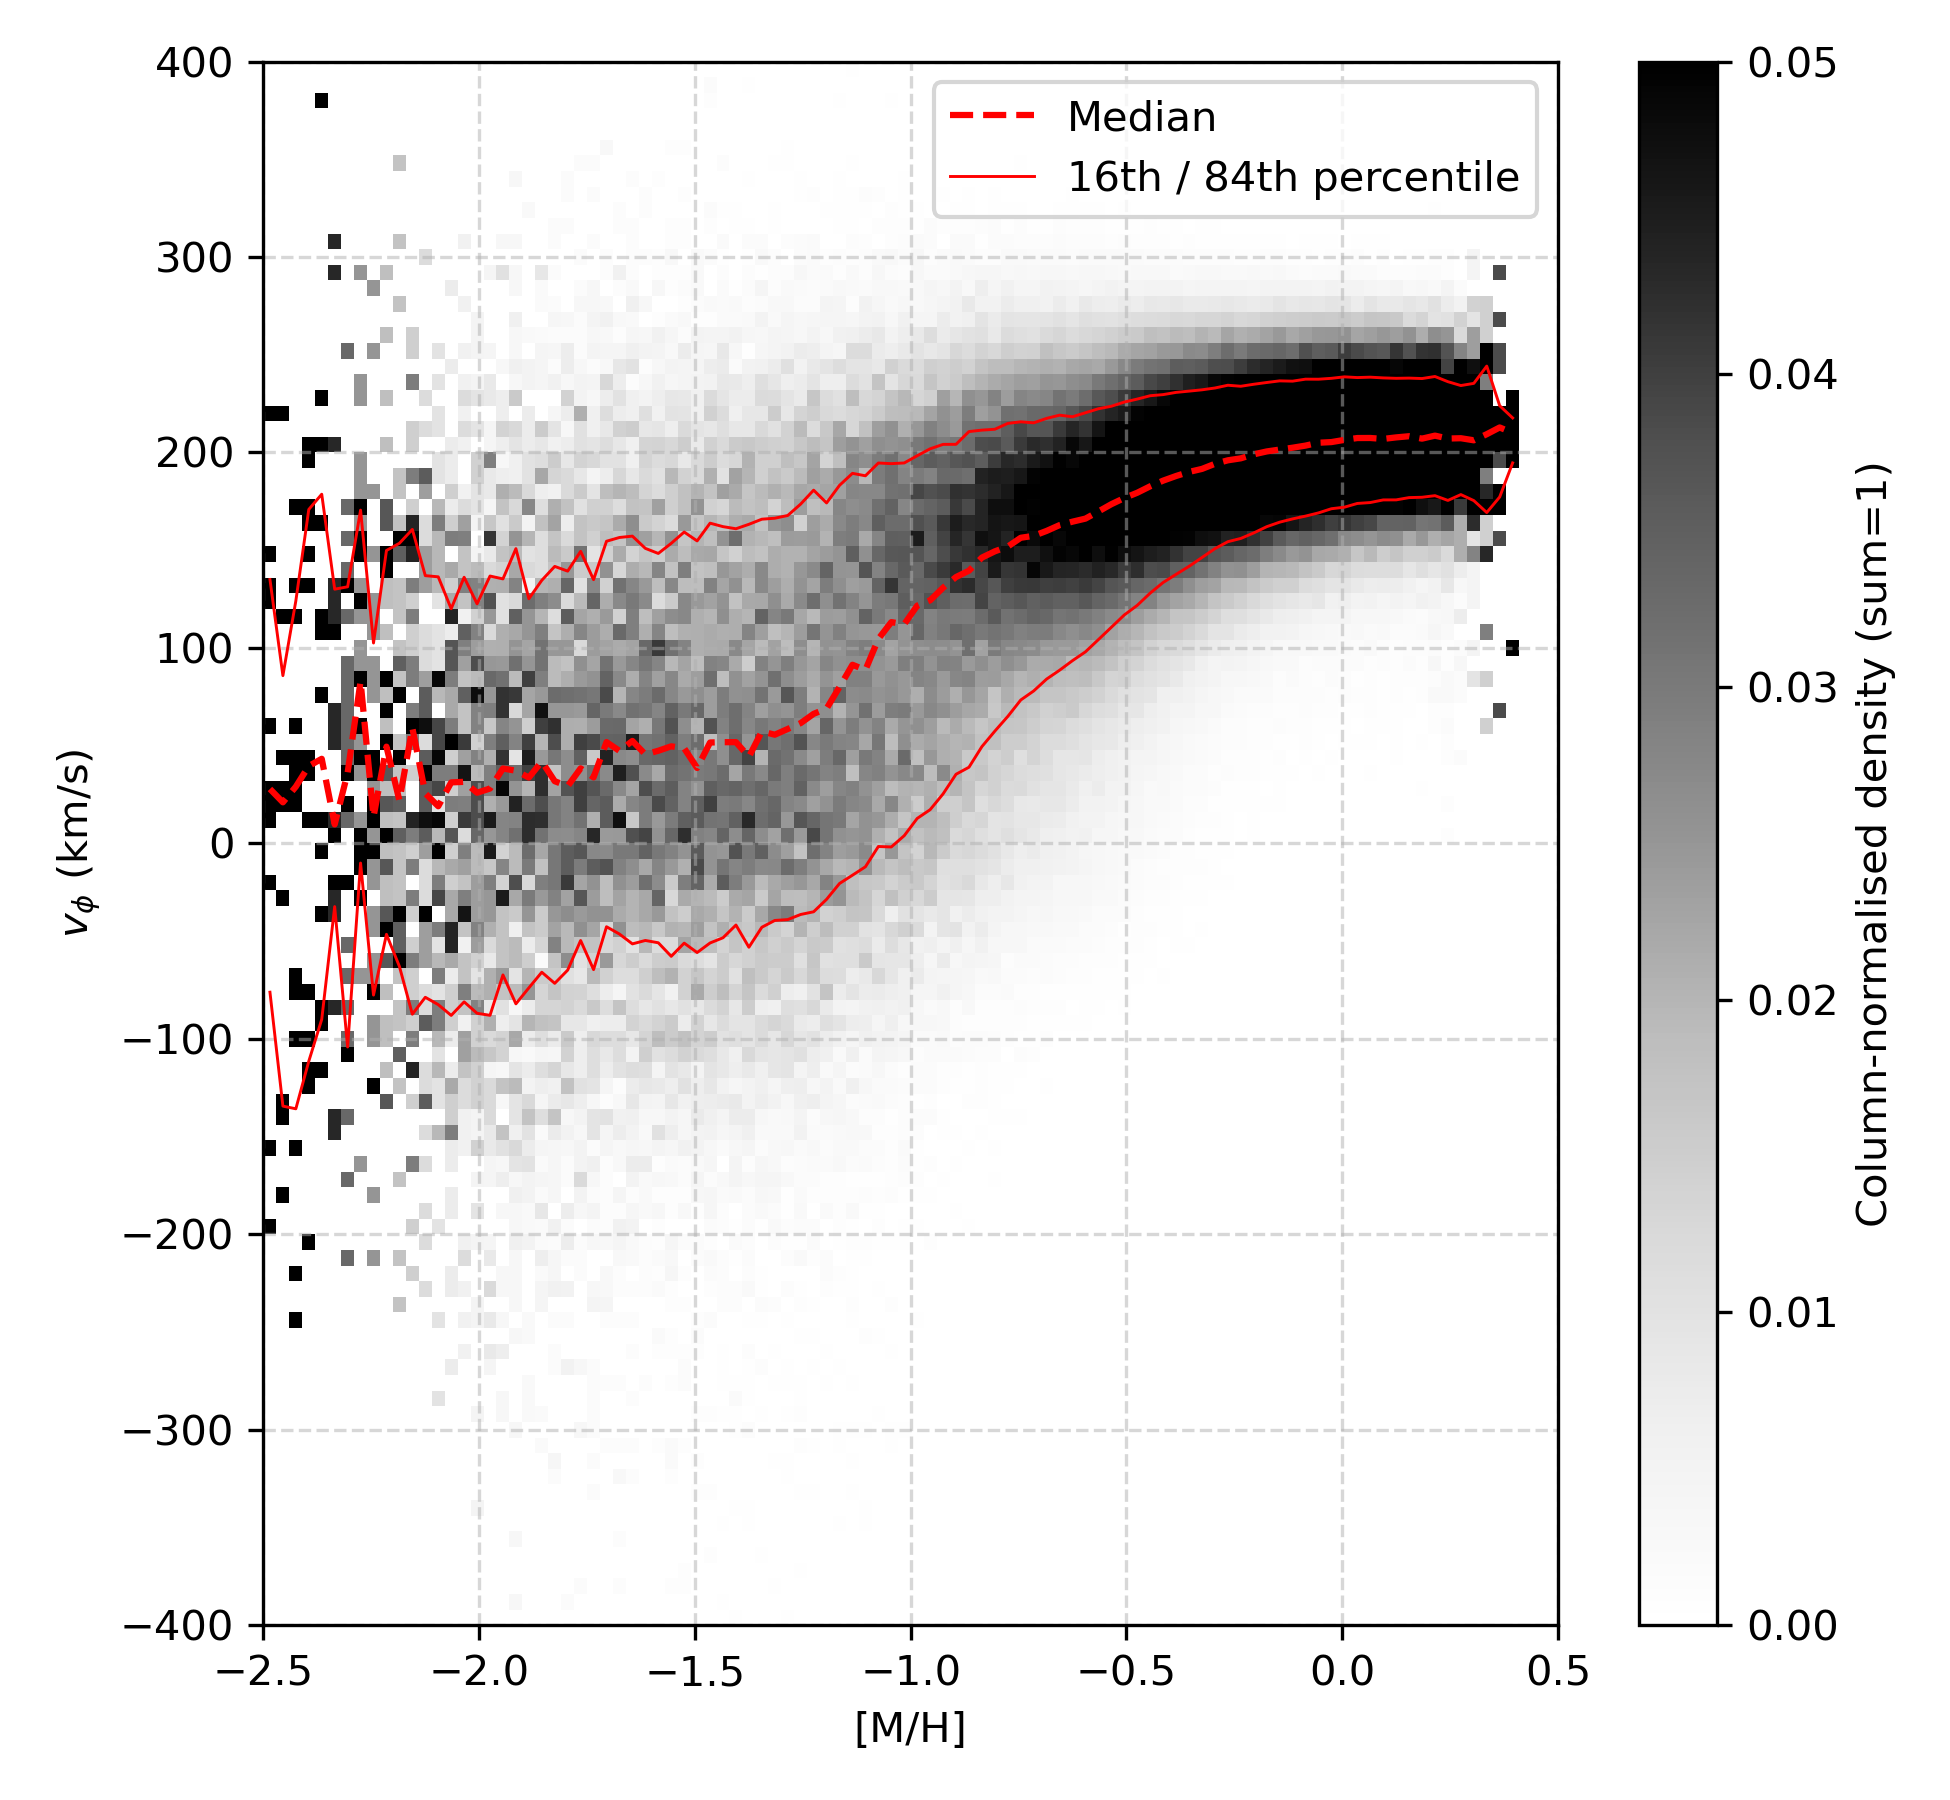
\includegraphics[width=\linewidth]{../figures/vis_mh_vphi_high_alpha.png}
    \caption{High $\alpha$ stars}
  \end{subfigure}
  \hfill
  \begin{subfigure}[t]{0.48\linewidth}
    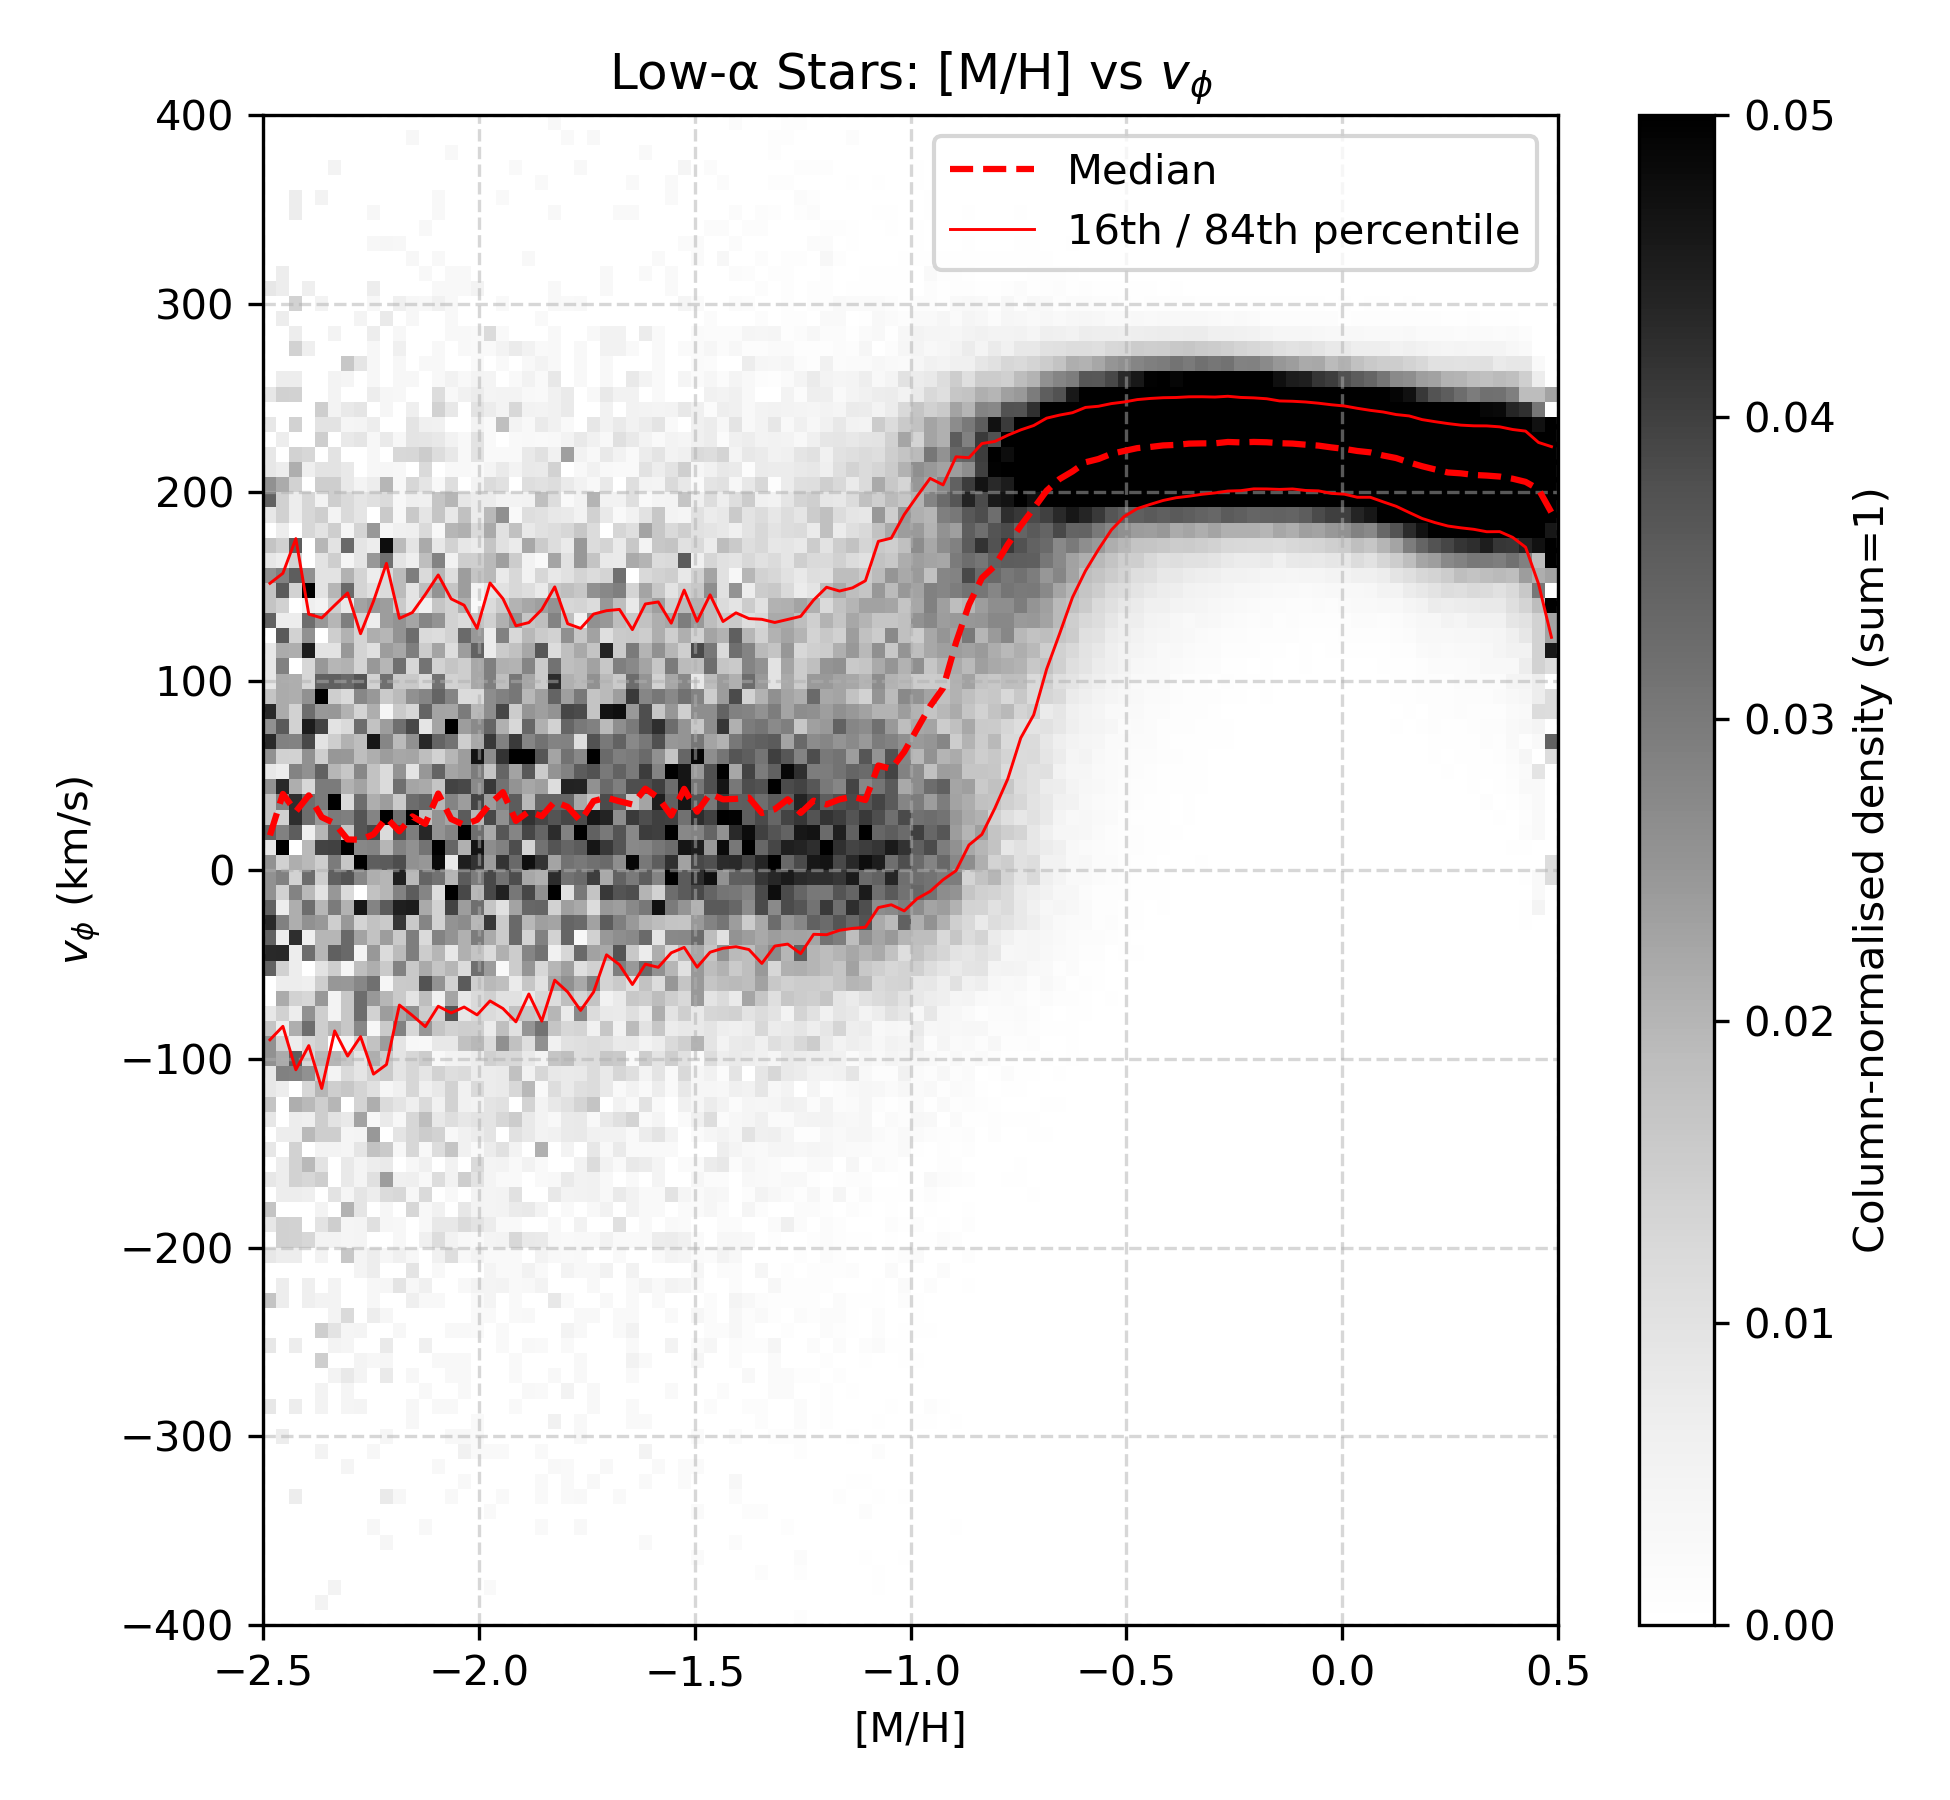
\includegraphics[width=\linewidth]{../figures/vis_mh_vphi_low_alpha.png}
    \caption{Low $\alpha$ stars}
  \end{subfigure}
  \caption{Median $v_\phi$ and dispersion vs.\ metallicity, split by $\alpha$-sequence.}
  \label{fig:mh_vphi_alpha}
\end{figure}

We applied XD-GMMs to the high and low $\alpha$ sequences separately (Figure~\ref{fig:gmm_alpha_bins}).  
In the \textit{high-$\alpha$} track, only a non-rotating halo is present at $\mathrm{[M/H]}\!\lesssim\!-2$.  
A thick-disc Gaussian first appears at $-1.6\!\lesssim\!\mathrm{[M/H]}\!\lesssim\!-1.3$, with $V_{\rm rot}/\sigma_{\phi}\!\approx\!2.4$.  
By $-1.3\!<\!\mathrm{[M/H]}\!<\!-1.0$ it grows to 52 \% and $V_{\rm rot}/\sigma_{\phi}\!\approx\!2.8$, indicating a gradual build-up of 
the thick disc from $\mathrm{[M/H]}\!\sim\!-1.6$.

\begin{figure}[H]
  \centering
  % Row 1
  \begin{subfigure}[t]{0.24\linewidth}
    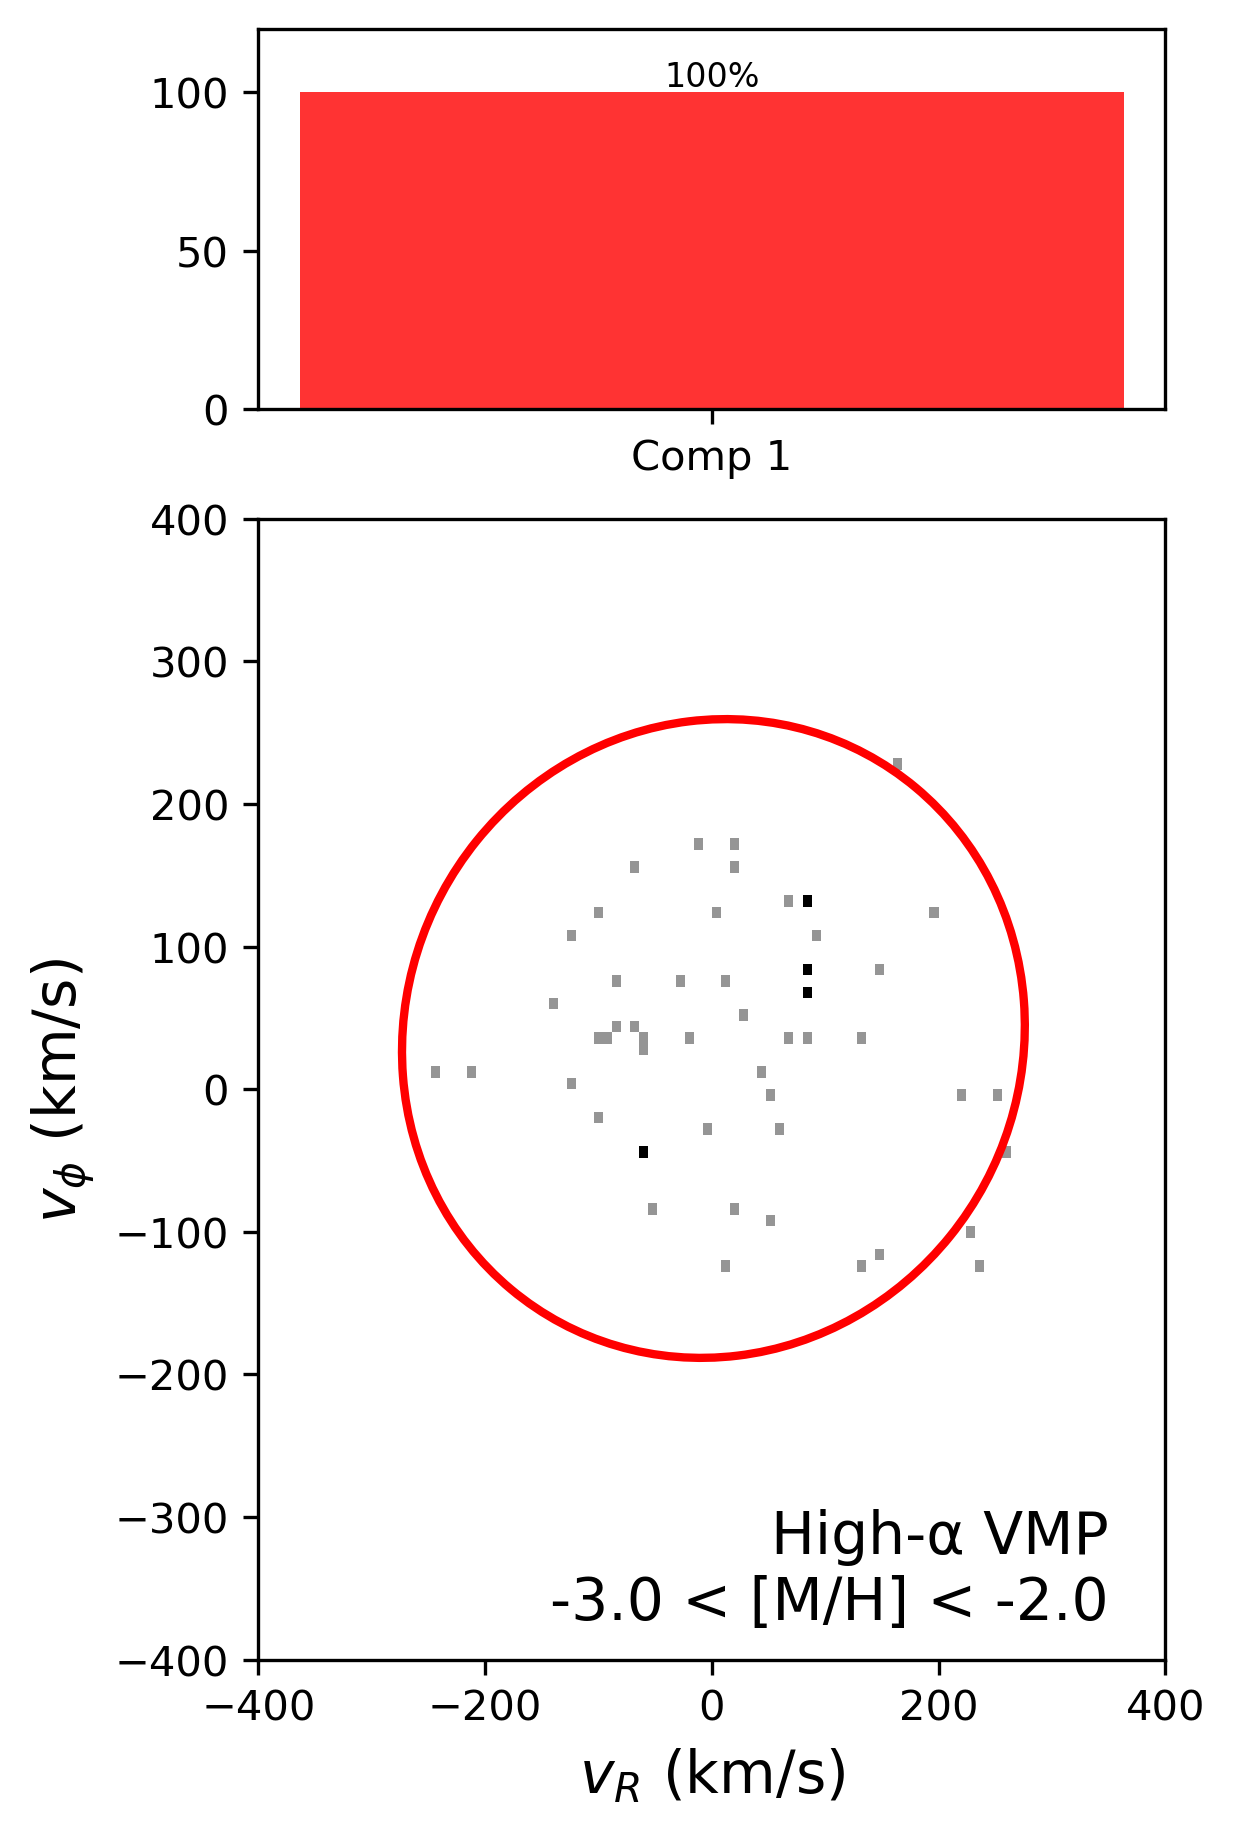
\includegraphics[width=\linewidth]{../figures/gmm_vmp_high_alpha_k1.png}
    \caption{\href{https://raw.githack.com/raunaq-rai/Disentangling-the-Milky-Way-using-GMM/main/figures/VMP\_high\_\_\_-3\%5BM\_H\%5D-2.html}{VMP $\alpha_{\mathrm{high}}$}}
    \label{fig:vmp_hi}
  \end{subfigure}\hfill
  \begin{subfigure}[t]{0.24\linewidth}
    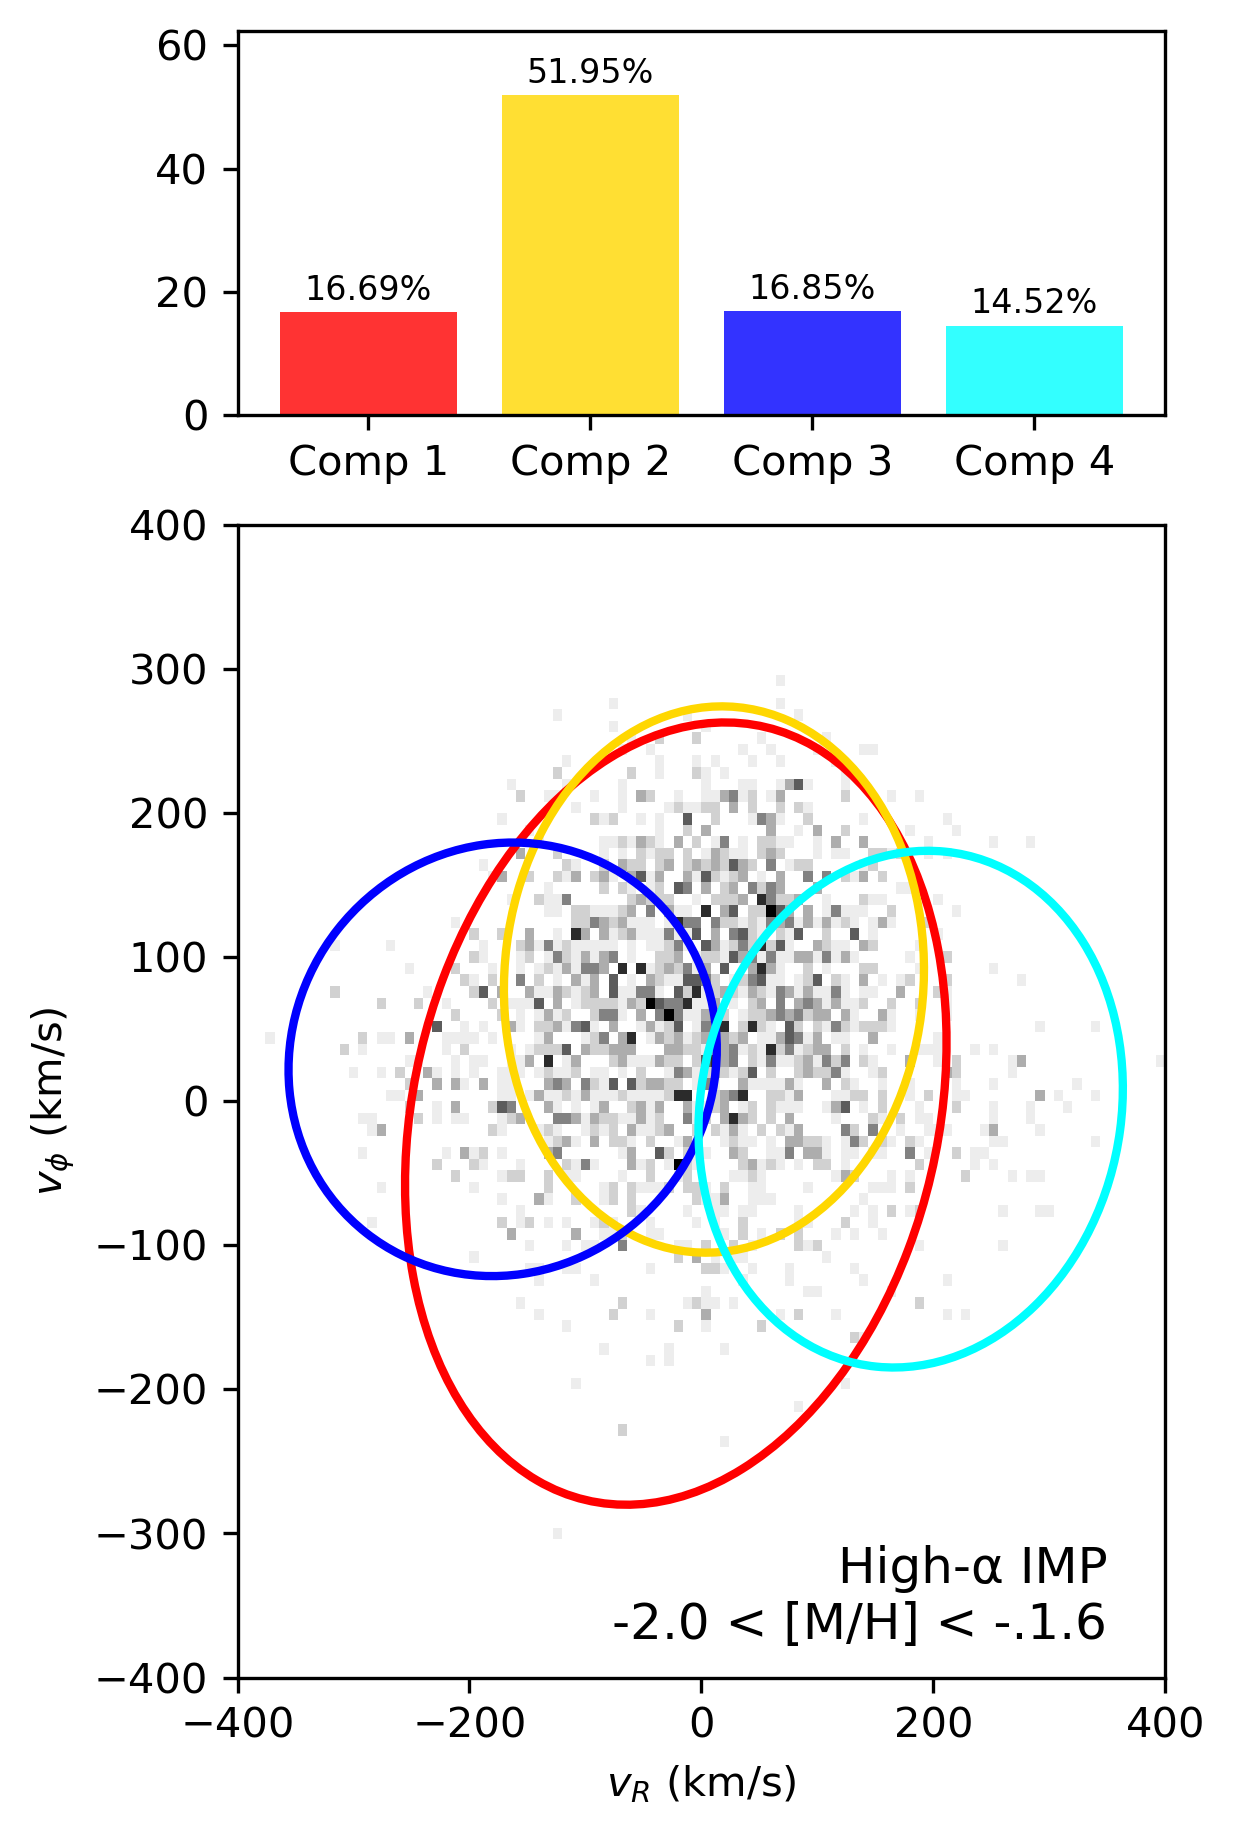
\includegraphics[width=\linewidth]{../figures/gmm_imp_high_alpha_k4.png}
    \caption{\href{https://raw.githack.com/raunaq-rai/Disentangling-the-Milky-Way-using-GMM/main/figures/IMP\_high\_\_\_-2\%5BM\_H\%5D-1.6.html}{IMP $\alpha_{\mathrm{high}}$}}
    \label{fig:imp_hi}
  \end{subfigure}\hfill
  \begin{subfigure}[t]{0.24\linewidth}
    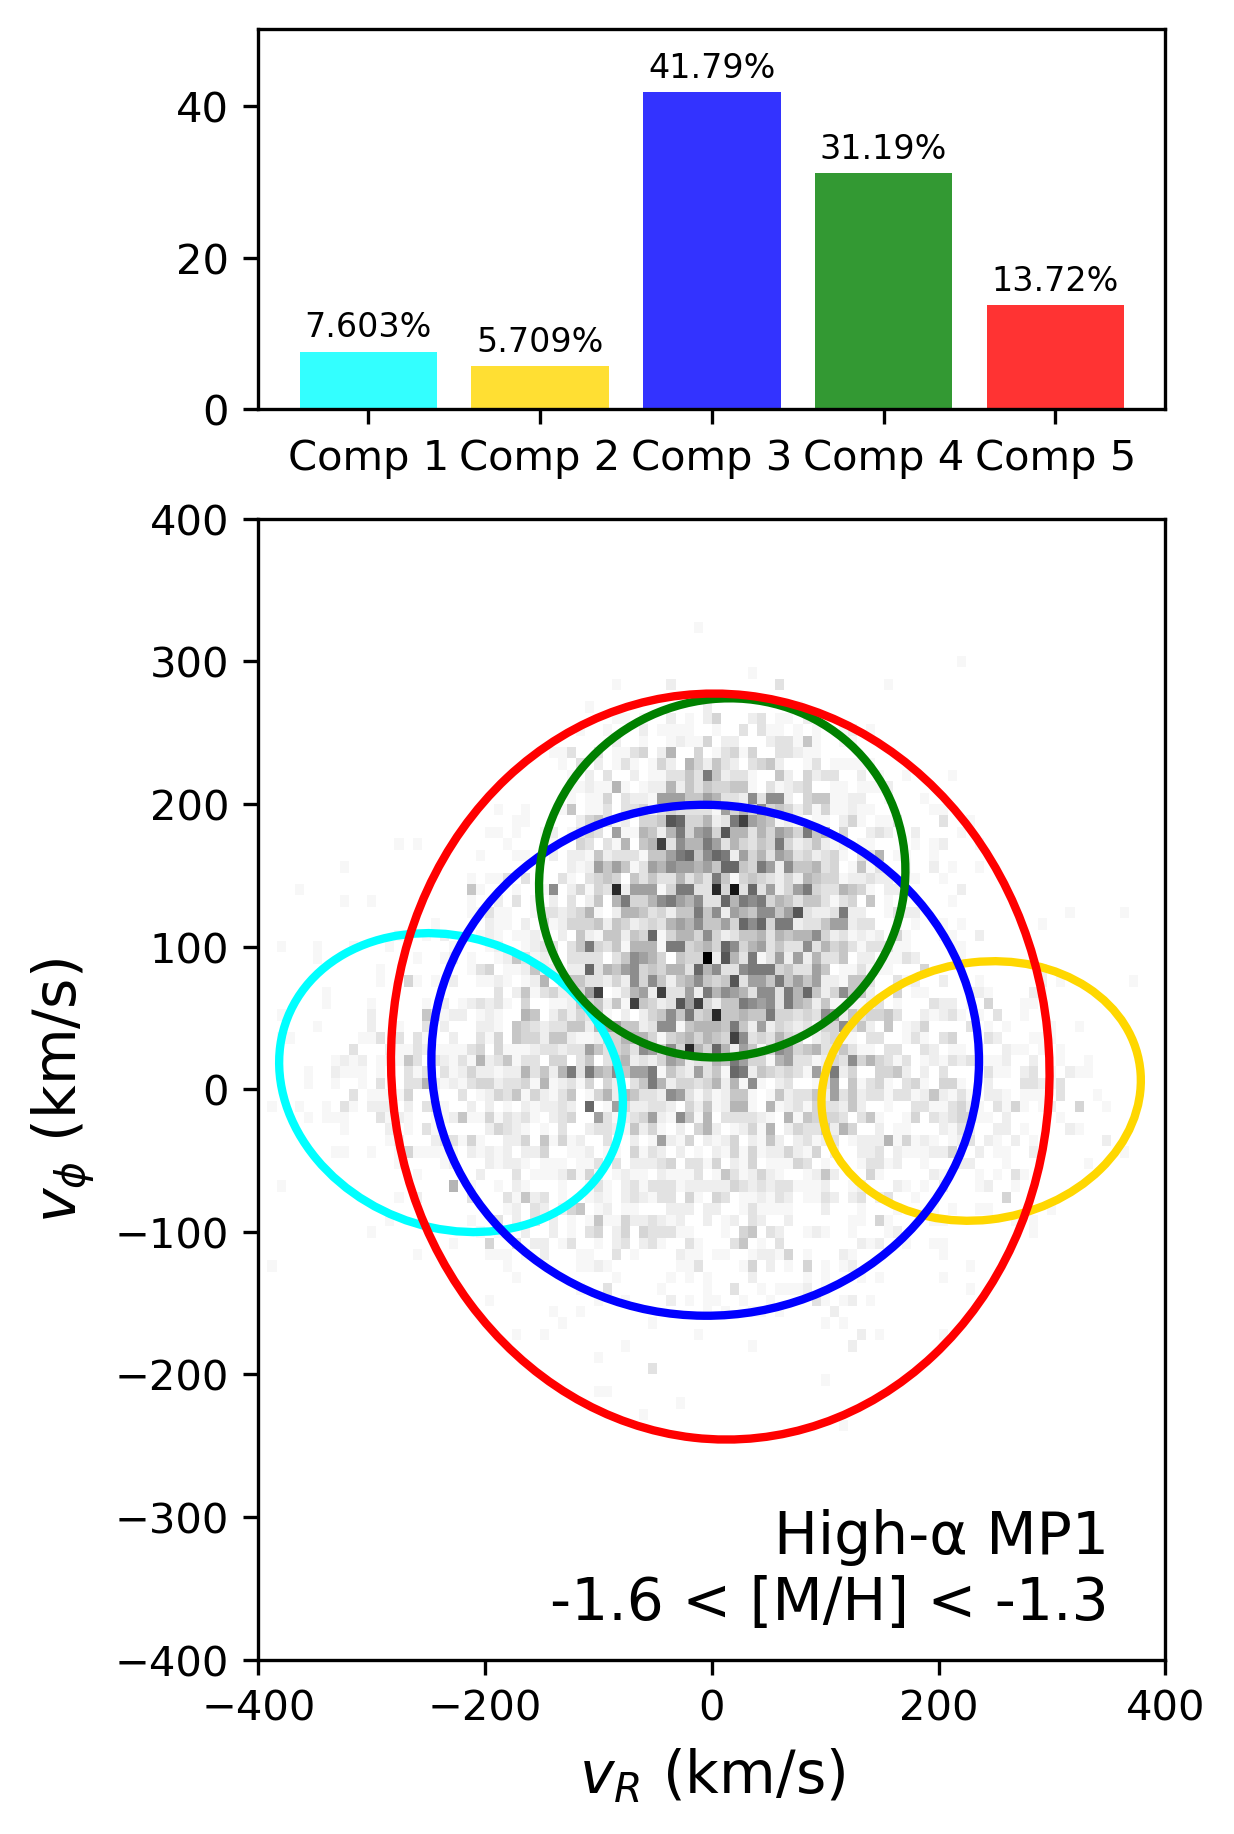
\includegraphics[width=\linewidth]{../figures/gmm_mp1_high_alpha_k5.png}
    \caption{\href{https://raw.githack.com/raunaq-rai/Disentangling-the-Milky-Way-using-GMM/main/figures/MP1\_high\_\_\_-1.6\%5BM\_H\%5D-1.3.html}{MP1 $\alpha_{\mathrm{high}}$}}
    \label{fig:mp1_hi}
  \end{subfigure}\hfill
  \begin{subfigure}[t]{0.24\linewidth}
    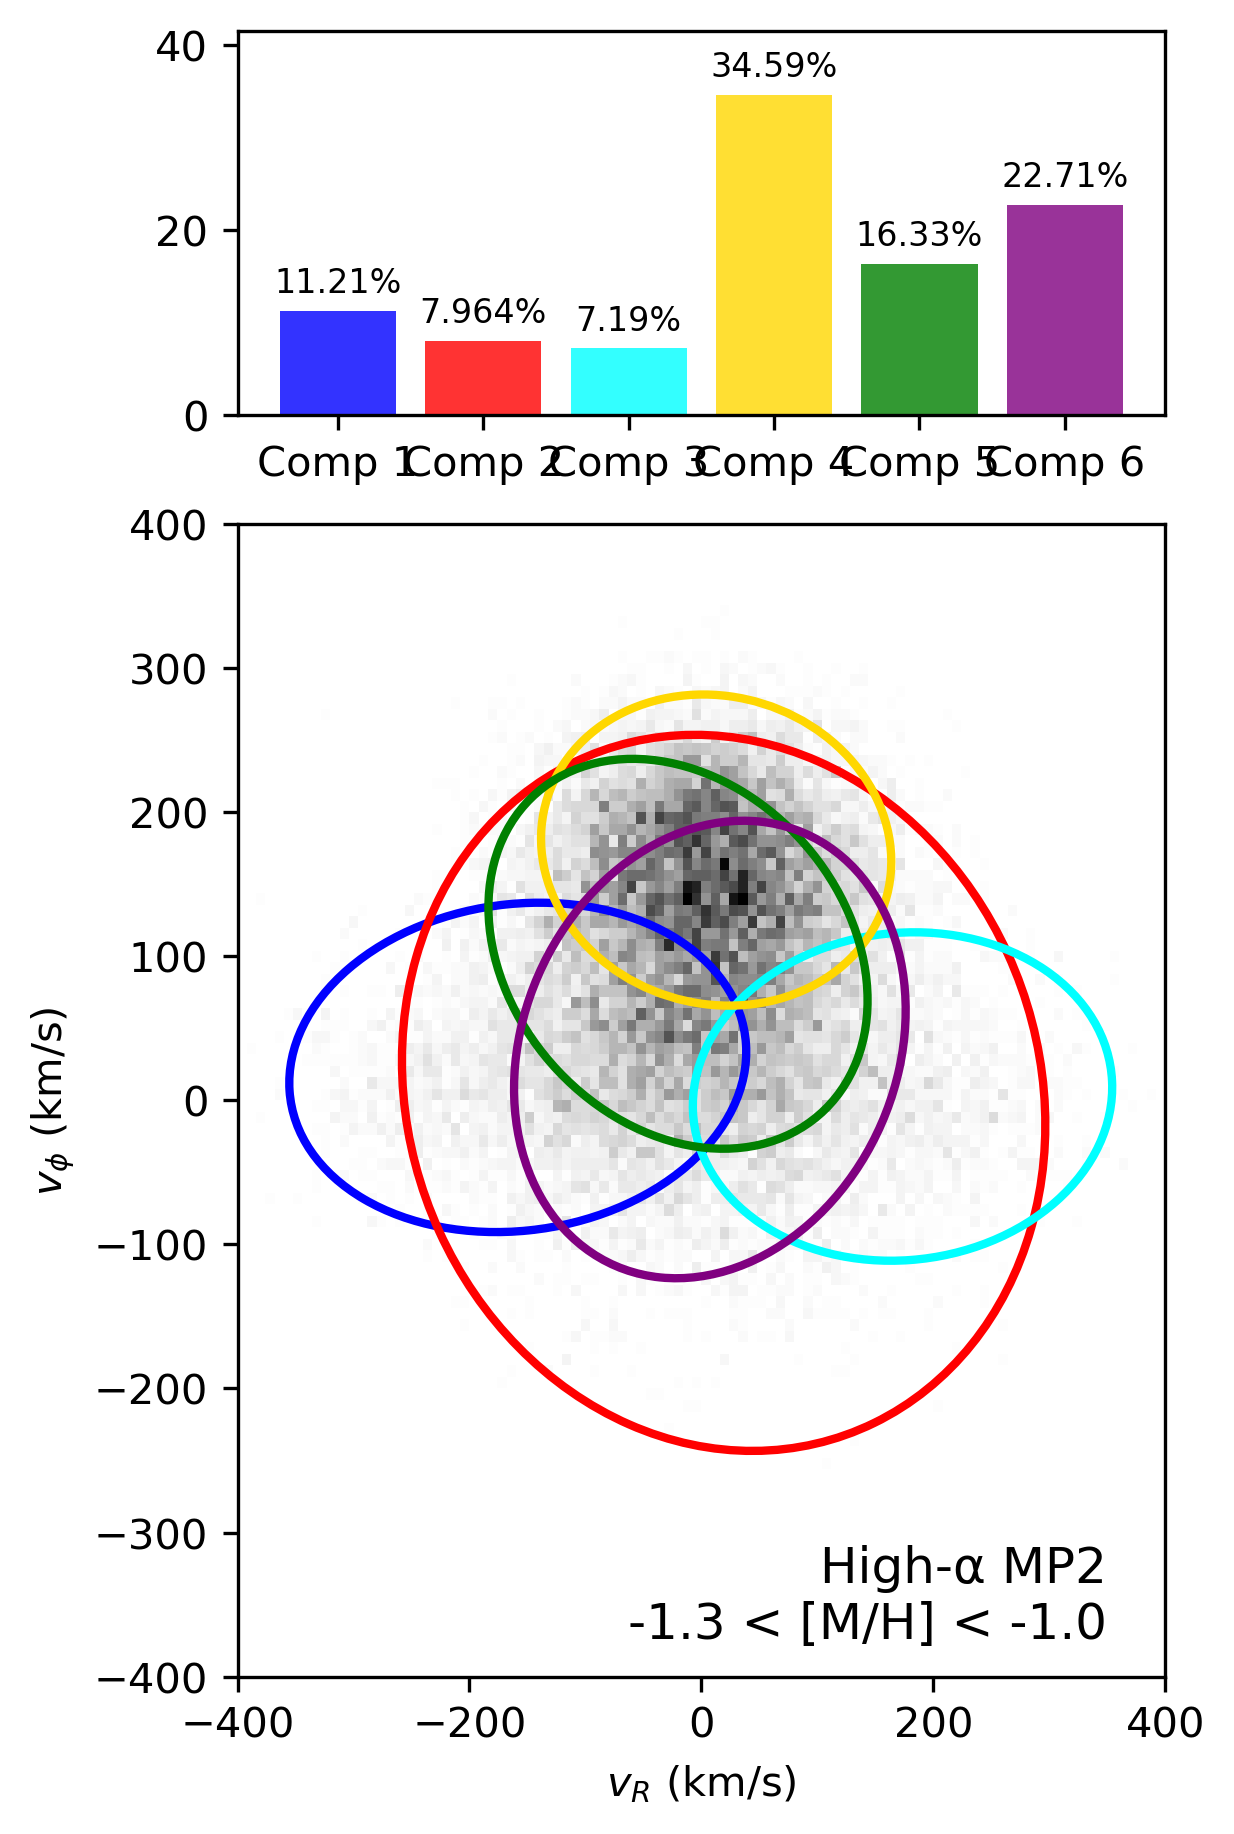
\includegraphics[width=\linewidth]{../figures/gmm_mp2_high_alpha_k6.png}
    \caption{\href{https://raw.githack.com/raunaq-rai/Disentangling-the-Milky-Way-using-GMM/main/figures/MP2\_high\_\_\_-1.3\%5BM\_H\%5D-1.0.html}{MP2 $\alpha_{\mathrm{high}}$}}
    \label{fig:mp2_hi}
  \end{subfigure}

  \vspace{0.5em}

  % Row 2: low-α (manual escapes)
  \begin{subfigure}[t]{0.24\linewidth}
    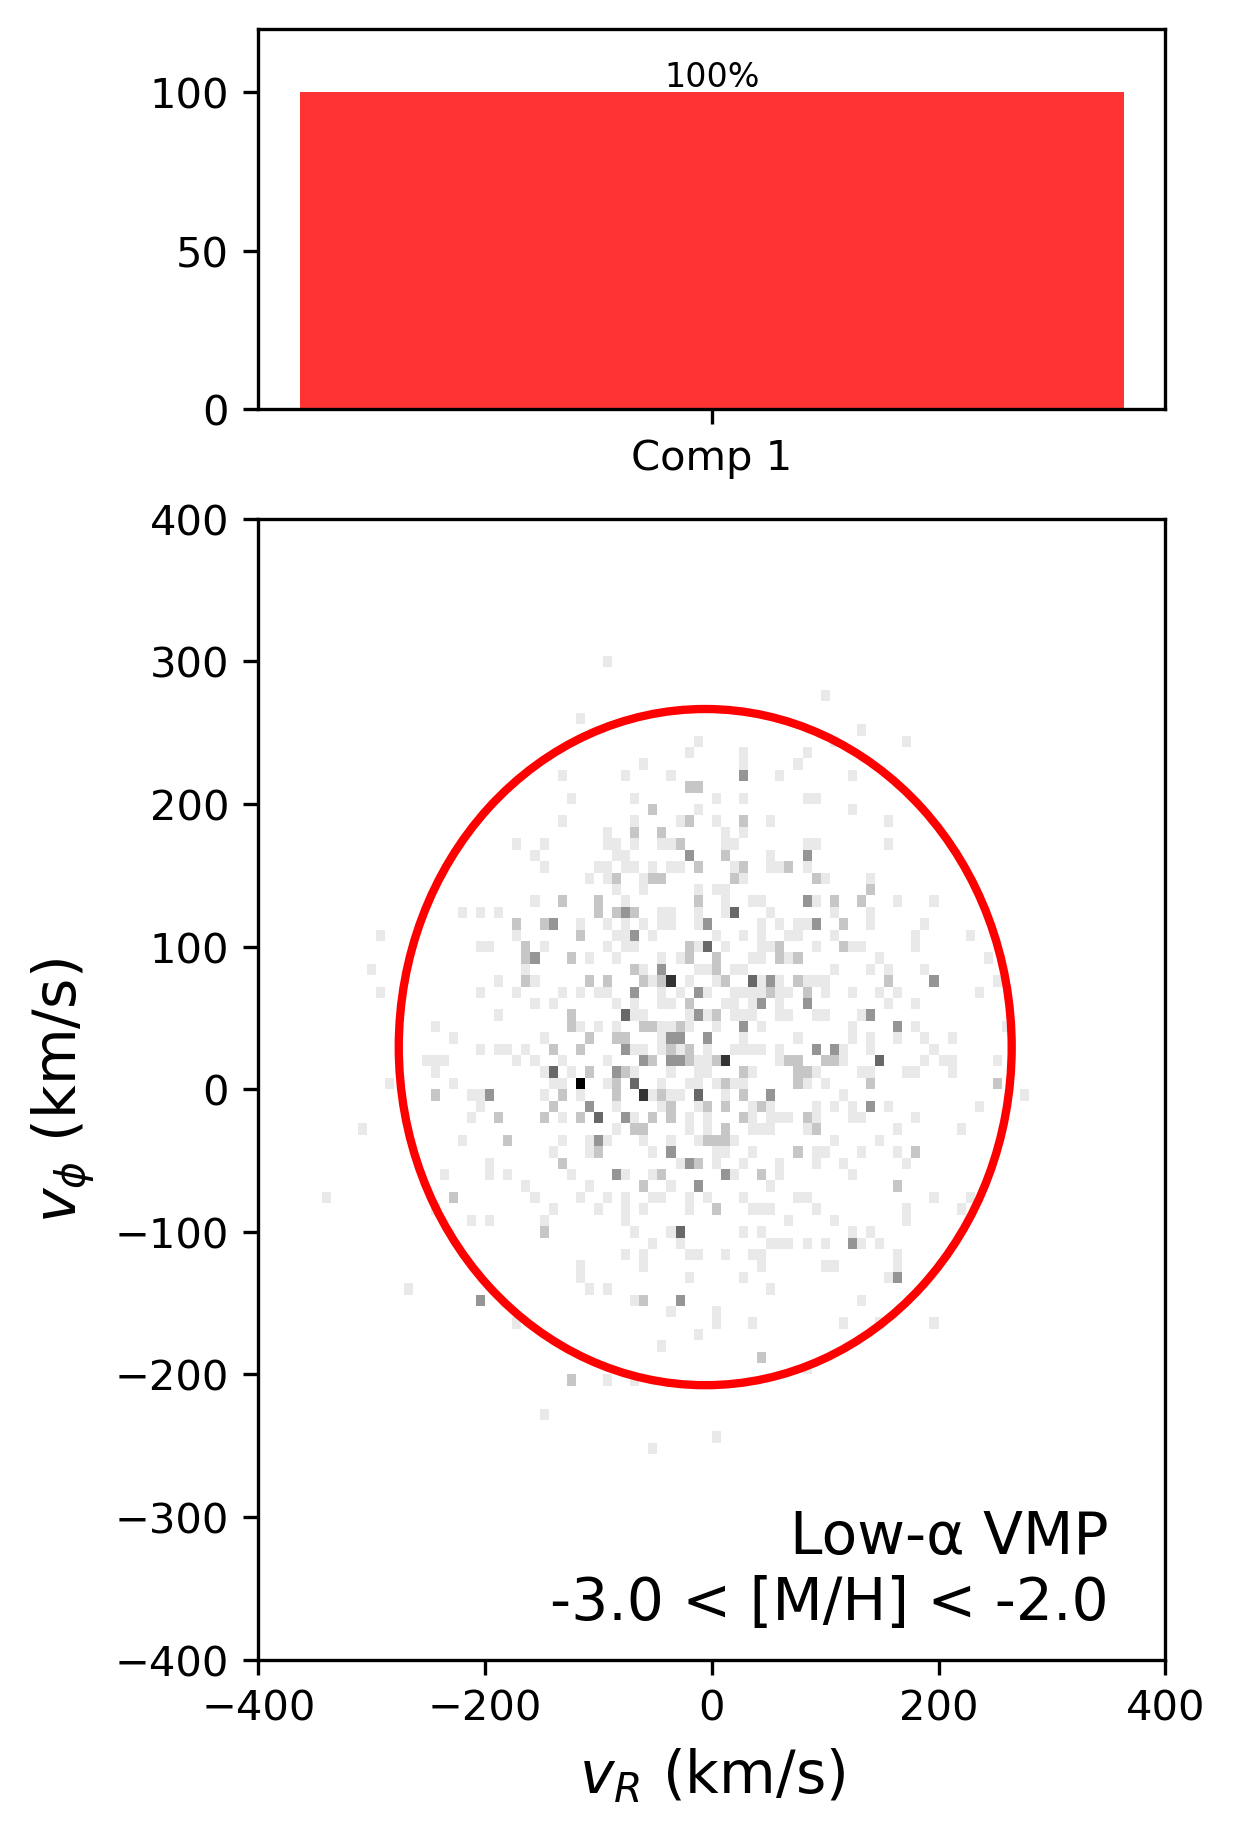
\includegraphics[width=\linewidth]{../figures/gmm_vmp_low_alpha_k1.png}
    \caption{\href{https://raw.githack.com/raunaq-rai/Disentangling-the-Milky-Way-using-GMM/main/figures/VMP\_low\_\_\_\_-3\%5BM\_H\%5D-2.html}{VMP $\alpha_{\mathrm{low}}$}}
    \label{fig:low_vmp}
  \end{subfigure}\hfill
  \begin{subfigure}[t]{0.24\linewidth}
    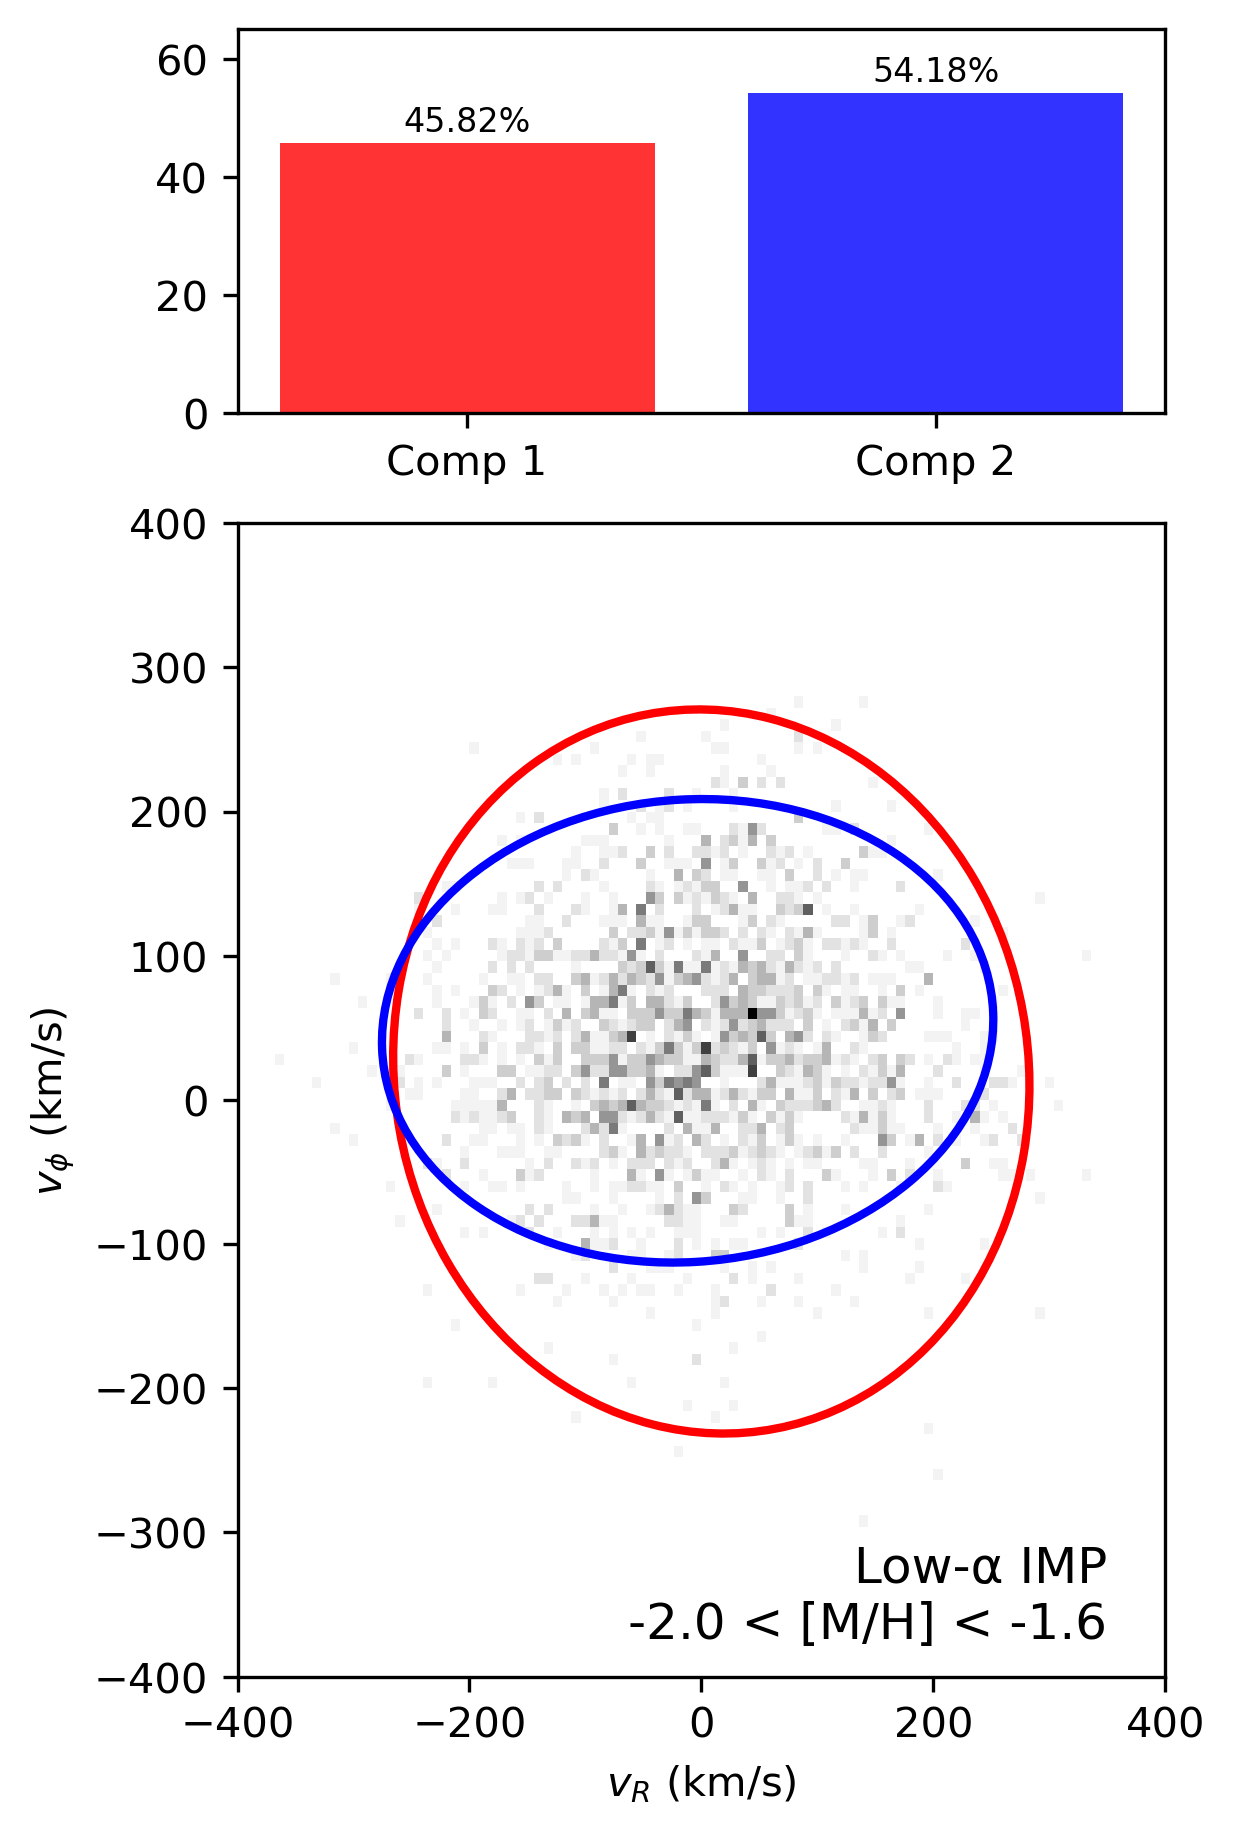
\includegraphics[width=\linewidth]{../figures/gmm_imp_low_alpha_k2.png}
    \caption{\href{https://raw.githack.com/raunaq-rai/Disentangling-the-Milky-Way-using-GMM/main/figures/IMP\_low\_\_\_\_-2\%5BM\_H\%5D-1.6.html}{IMP $\alpha_{\mathrm{low}}$}}
    \label{fig:low_imp}
  \end{subfigure}\hfill
  \begin{subfigure}[t]{0.24\linewidth}
    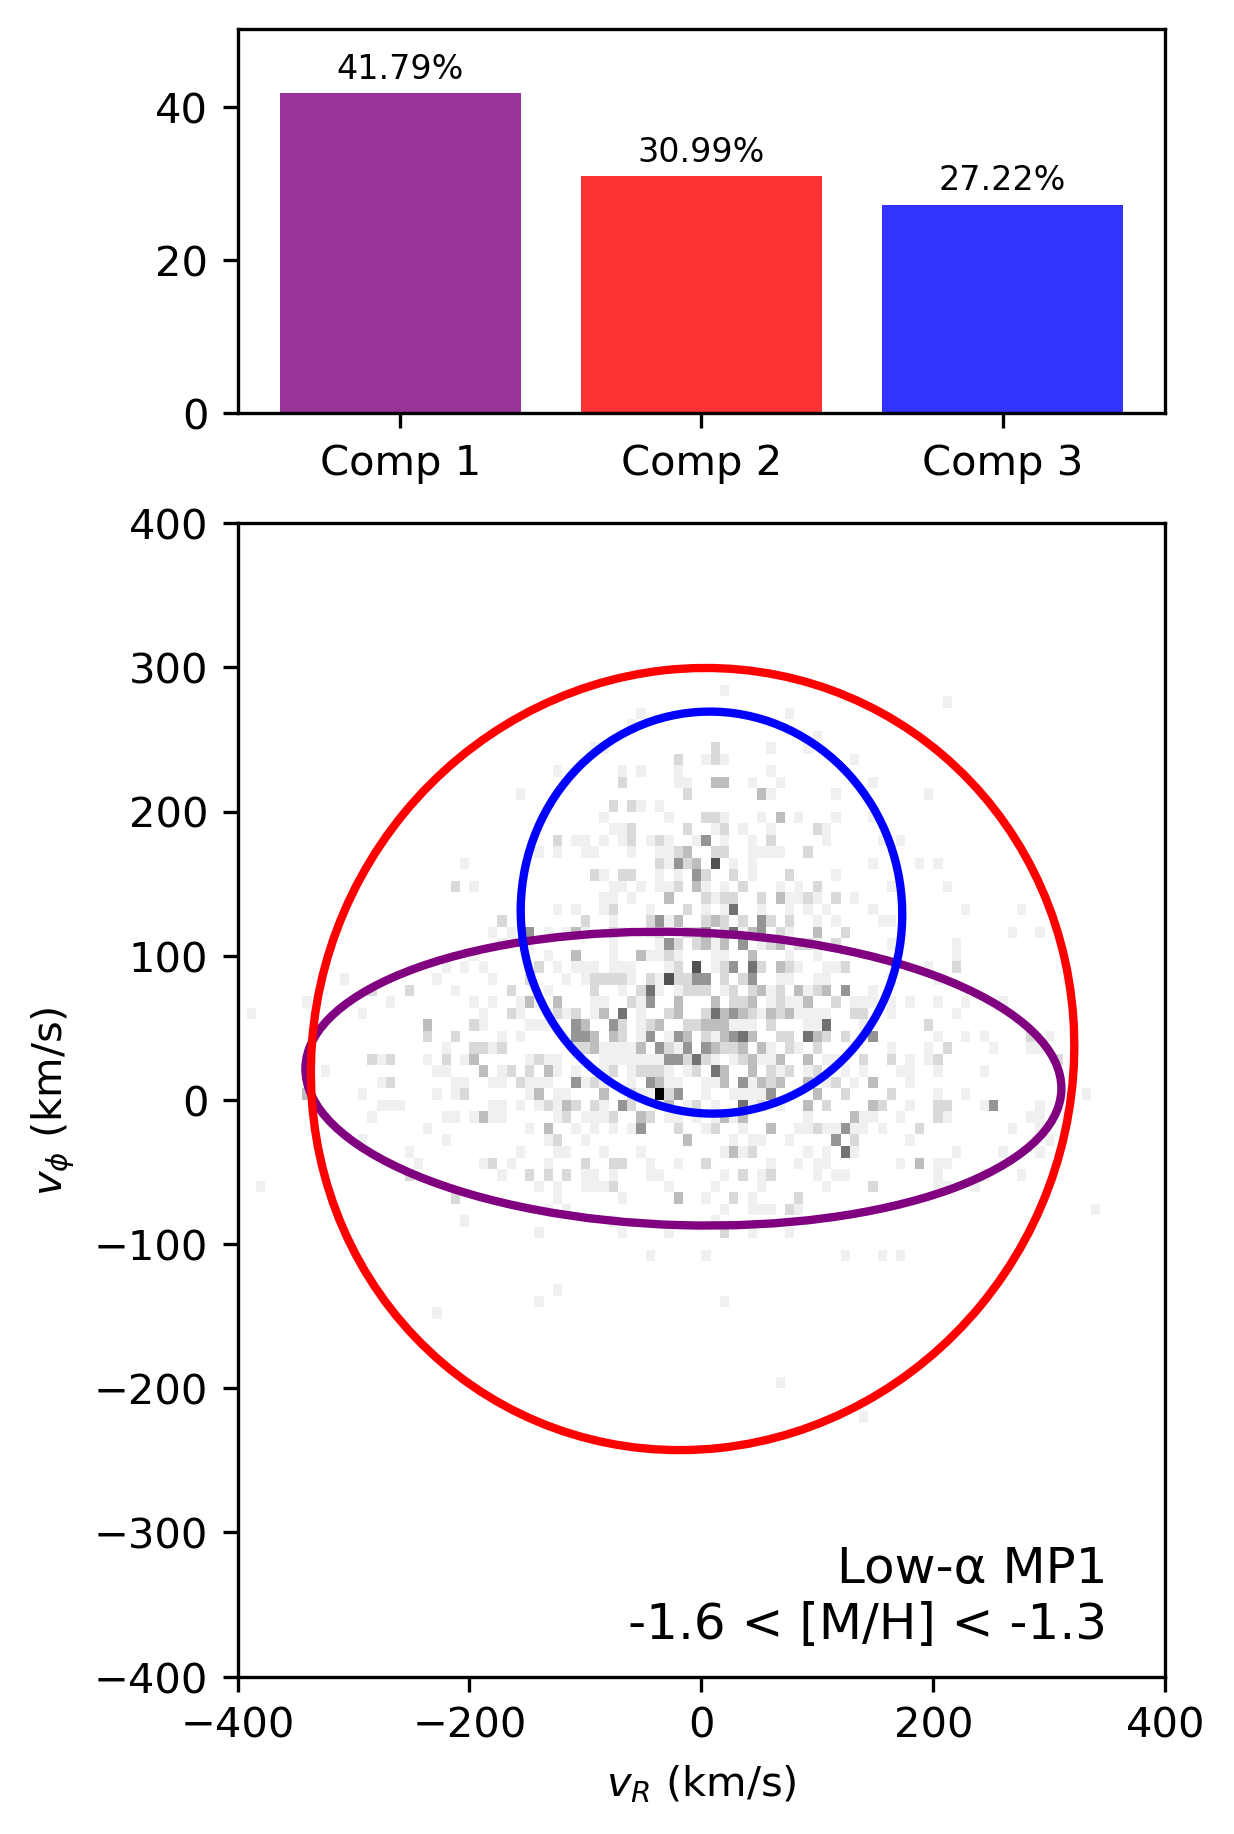
\includegraphics[width=\linewidth]{../figures/gmm_mp1_low_alpha_k4.png}
    \caption{\href{https://raw.githack.com/raunaq-rai/Disentangling-the-Milky-Way-using-GMM/main/figures/MP1\_low\_\_\_\_-1.6\%5BM\_H\%5D-1.3.html}{MP1 $\alpha_{\mathrm{low}}$}}
    \label{fig:low_mp1}
  \end{subfigure}\hfill
  \begin{subfigure}[t]{0.24\linewidth}
    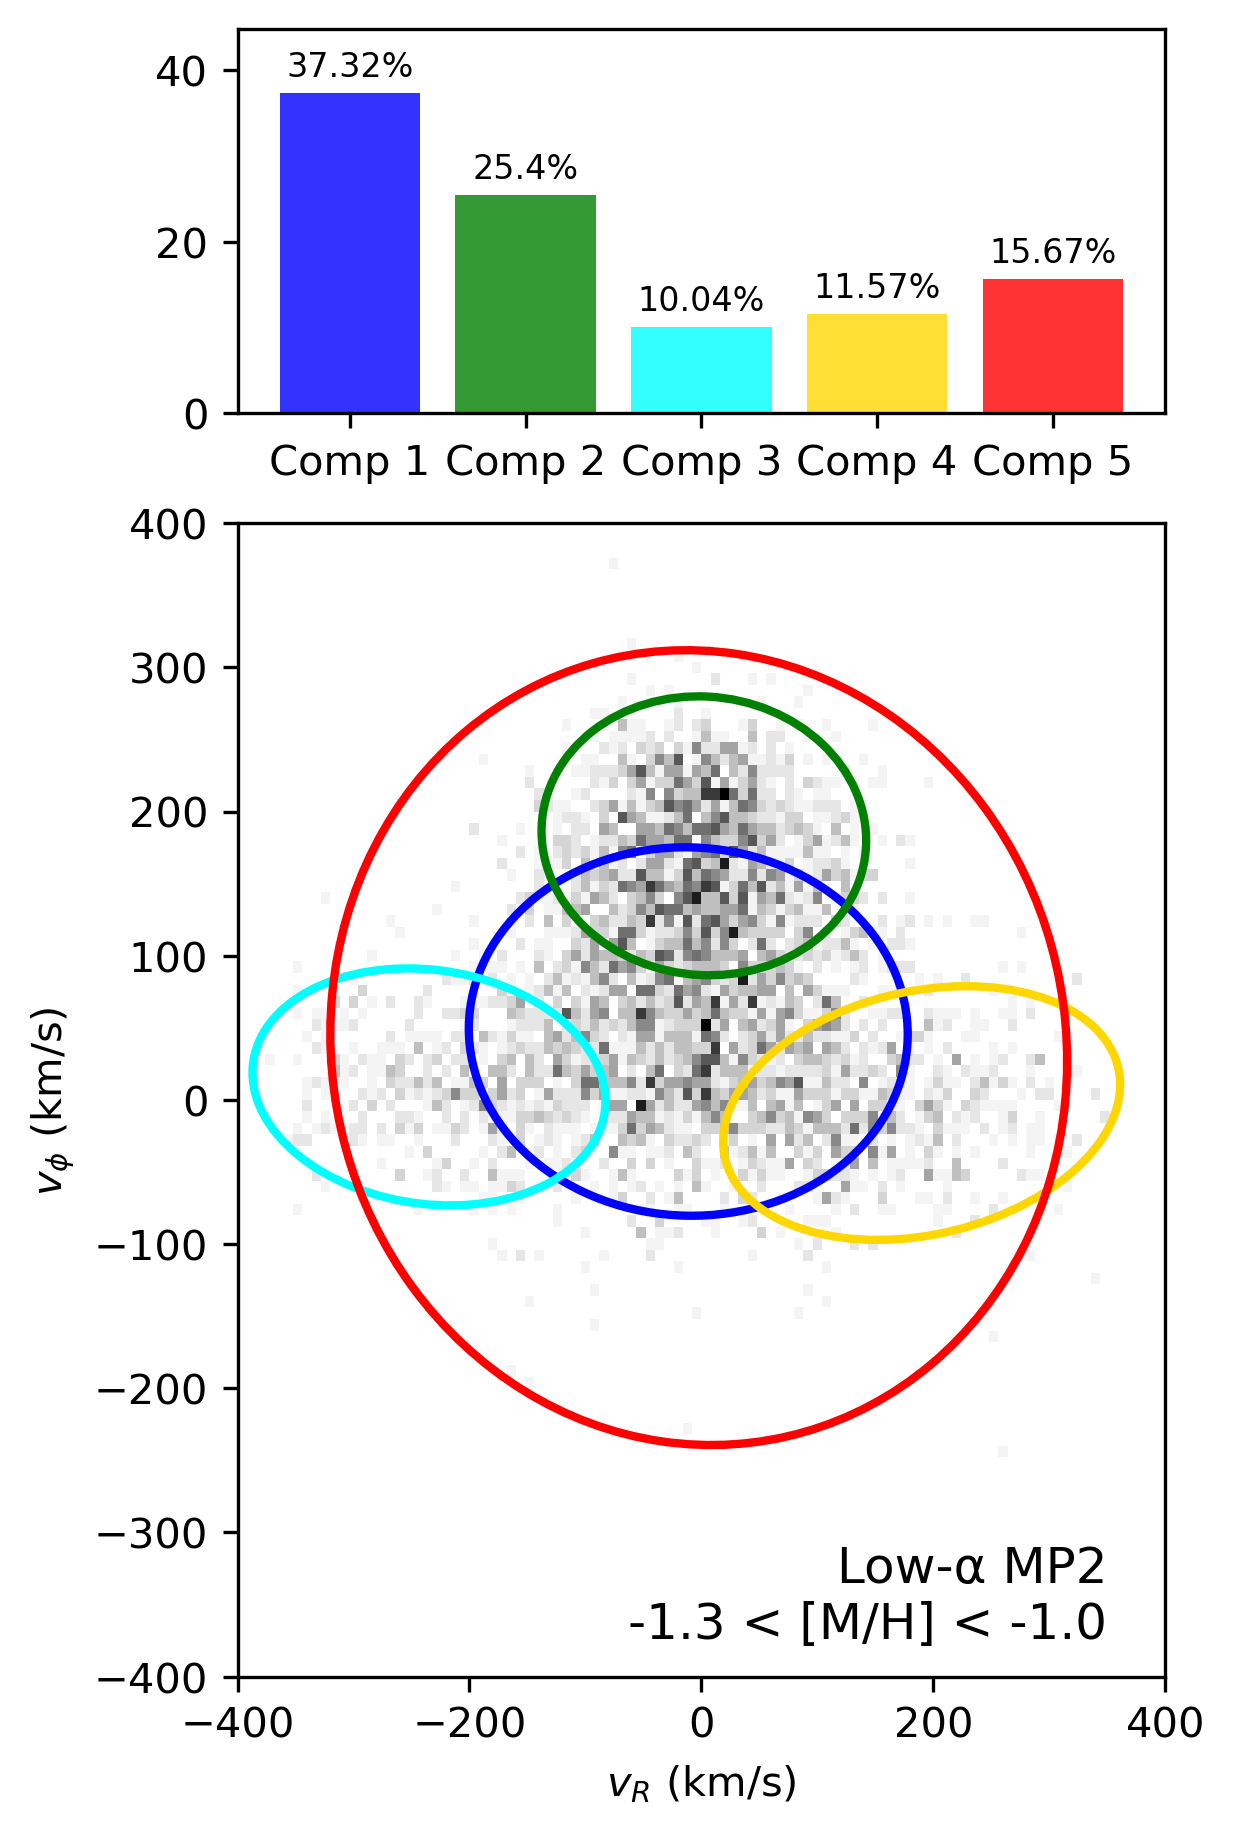
\includegraphics[width=\linewidth]{../figures/gmm_mp2_low_alpha_k6.png}
    \caption{\href{https://raw.githack.com/raunaq-rai/Disentangling-the-Milky-Way-using-GMM/main/figures/MP2\_low\_\_\_\_-1.3\%5BM\_H\%5D-1.0.html}{MP2 $\alpha_{\mathrm{low}}$}}
    \label{fig:low_mp2}
  \end{subfigure}


  \caption{XD-GMM decomposition across $\alpha$-sequences and metallicity bins. Top row: high-$\alpha$; bottom row: low-$\alpha$.}
  \label{fig:gmm_alpha_bins}
\end{figure}

In the \textit{low-$\alpha$} branch, a thick‐disc component (25\% of stars) only appears in the MP2 
bin ($-1.3<\mathrm{[M/H]}<-1.0$), but its high $V_{\rm rot}/\sigma_{\phi}\approx3.8$, above 
the $\sim3$ discy threshold, suggests contamination by a colder thin‐disc population. We do not observe
a thin disc in the low-$\alpha$ sequence as expected due to sample selection effects.

GS/E-like radial Gaussians appear in both sequences, probably due to misclassified $\alpha$-poor debris, underscoring the need for robust chemical labelling.  
Overall, the high-$\alpha$ thick disc assembled earlier and gradually (\mbox{$\mathrm{[M/H]}\!\gtrsim\!-1.6$}), while the low-$\alpha$ thin disc formed later and swiftly (\mbox{$\mathrm{[M/H]}\!\gtrsim\!-1.3$}).



\section*{Recommendations and Next Steps}

\begin{itemize}
\item \textbf{Richer dynamical models.} Replace Gaussian mixtures with distribution-function or action-based models to capture non-Gaussian and asymmetric structures.  
\item \textbf{Tighter chemistry.} Improve $\alpha$–abundance precision (or use high-resolution follow-up) to reduce sequence cross-contamination, especially at low metallicity.  
\item \textbf{Explicit selection function.} Model Gaia’s magnitude and colour cuts to convert component weights into unbiased population fractions.  
\item \textbf{GS/E contamination.} Re-examine the high-$\alpha$ bins with stricter chemical cuts to confirm whether the apparent GS/E signatures are real or artefacts.  
\end{itemize}

\section*{Conclusion and Research Impact}

Splitting Gaia DR3 red giants by $\alpha$ abundance reveals a \emph{two-phase} disc build-up:  
the high-$\alpha$ sequence gains rotational support at $\mathrm{[M/H]}\!\approx\!-1.6$, forming 
a thick disc that grows gradually, while the low-$\alpha$ sequence does not reach disc 
kinematics until $\mathrm{[M/H]}\!\approx\!-1.3$. This confirms that no metal-poor 
($\mathrm{[M/H]}\!<\!-2$) disc exists and clarifies the distinct evolutionary paths of 
the thick and thin discs.  

Coupling precise chemistry with full 3-D kinematics provides a template for forthcoming surveys 
(WEAVE, 4MOST, SDSS-V) to isolate, date and map Milky-Way disc components. Pinpointing the 
metallicity–$\alpha$ thresholds for disc formation tightens constraints on early star-formation, 
feedback and merger heating in disc galaxies, advancing our reconstruction of the Galaxy’s 
assembly history.  


\newpage{}

965 / 1000 words








\bibliographystyle{unsrt}  
\bibliography{references}

% End of two-column content
\end{multicols}



\end{document}
